\documentclass[a4paper,12pt,twoside]{memoir}

% Castellano
\usepackage[spanish,es-tabla]{babel}
\selectlanguage{spanish}
\usepackage[utf8]{inputenc}
\usepackage[T1]{fontenc}
\usepackage{lmodern} % Scalable font
\usepackage{microtype}
\usepackage{placeins}


\RequirePackage{booktabs}
\RequirePackage[table]{xcolor}
\RequirePackage{xtab}
\RequirePackage{multirow}

% Links
\PassOptionsToPackage{hyphens}{url}\usepackage[colorlinks]{hyperref}
\hypersetup{
	allcolors = {red}
}

% Ecuaciones
\usepackage{amsmath}

% Mis estilos
\usepackage{makecell}
\usepackage{amssymb}
\usepackage{float}
\usepackage{tikz}
\usetikzlibrary{matrix}
\usetikzlibrary{shapes, positioning}

\usepackage{pdflscape}
\usepackage{tabularx}
\usepackage{array}
\usepackage{subcaption}


% Rutas de fichero / paquete
\newcommand{\ruta}[1]{{\sffamily #1}}

% Párrafos
\nonzeroparskip

% Huérfanas y viudas
\widowpenalty100000
\clubpenalty100000

% Imágenes

% Comando para insertar una imagen en un lugar concreto.
% Los parámetros son:
% 1 --> Ruta absoluta/relativa de la figura
% 2 --> Texto a pie de figura
% 3 --> Tamaño en tanto por uno relativo al ancho de página
\usepackage{graphicx}
\newcommand{\imagen}[3]{
	\begin{figure}[!h]
		\centering
		\includegraphics[width=#3\textwidth]{#1}
		\caption{#2}\label{fig:#1}
	\end{figure}
	\FloatBarrier
}

% Comando para insertar una imagen sin posición.
% Los parámetros son:
% 1 --> Ruta absoluta/relativa de la figura
% 2 --> Texto a pie de figura
% 3 --> Tamaño en tanto por uno relativo al ancho de página
\newcommand{\imagenflotante}[3]{
	\begin{figure}
		\centering
		\includegraphics[width=#3\textwidth]{#1}
		\caption{#2}\label{fig:#1}
	\end{figure}
}

% El comando \figura nos permite insertar figuras comodamente, y utilizando
% siempre el mismo formato. Los parametros son:
% 1 --> Porcentaje del ancho de página que ocupará la figura (de 0 a 1)
% 2 --> Fichero de la imagen
% 3 --> Texto a pie de imagen
% 4 --> Etiqueta (label) para referencias
% 5 --> Opciones que queramos pasarle al \includegraphics
% 6 --> Opciones de posicionamiento a pasarle a \begin{figure}
\newcommand{\figuraConPosicion}[6]{%
  \setlength{\anchoFloat}{#1\textwidth}%
  \addtolength{\anchoFloat}{-4\fboxsep}%
  \setlength{\anchoFigura}{\anchoFloat}%
  \begin{figure}[#6]
    \begin{center}%
      \Ovalbox{%
        \begin{minipage}{\anchoFloat}%
          \begin{center}%
            \includegraphics[width=\anchoFigura,#5]{#2}%
            \caption{#3}%
            \label{#4}%
          \end{center}%
        \end{minipage}
      }%
    \end{center}%
  \end{figure}%
}

%
% Comando para incluir imágenes en formato apaisado (sin marco).
\newcommand{\figuraApaisadaSinMarco}[5]{%
  \begin{figure}%
    \begin{center}%
    \includegraphics[angle=90,height=#1\textheight,#5]{#2}%
    \caption{#3}%
    \label{#4}%
    \end{center}%
  \end{figure}%
}
% Para las tablas
\newcommand{\otoprule}{\midrule [\heavyrulewidth]}
%
% Nuevo comando para tablas pequeñas (menos de una página).
\newcommand{\tablaSmall}[5]{%
 \begin{table}
  \begin{center}
   \rowcolors {2}{gray!35}{}
   \begin{tabular}{#2}
    \toprule
    #4
    \otoprule
    #5
    \bottomrule
   \end{tabular}
   \caption{#1}
   \label{tabla:#3}
  \end{center}
 \end{table}
}

%
% Nuevo comando para tablas pequeñas (menos de una página).
\newcommand{\tablaSmallSinColores}[5]{%
 \begin{table}[H]
  \begin{center}
   \begin{tabular}{#2}
    \toprule
    #4
    \otoprule
    #5
    \bottomrule
   \end{tabular}
   \caption{#1}
   \label{tabla:#3}
  \end{center}
 \end{table}
}

\newcommand{\tablaApaisadaSmall}[5]{%
\begin{landscape}
  \begin{table}
   \begin{center}
    \rowcolors {2}{gray!35}{}
    \begin{tabular}{#2}
     \toprule
     #4
     \otoprule
     #5
     \bottomrule
    \end{tabular}
    \caption{#1}
    \label{tabla:#3}
   \end{center}
  \end{table}
\end{landscape}
}

%
% Nuevo comando para tablas grandes con cabecera y filas alternas coloreadas en gris.
\newcommand{\tabla}[6]{%
  \begin{center}
    \tablefirsthead{
      \toprule
      #5
      \otoprule
    }
    \tablehead{
      \multicolumn{#3}{l}{\small\sl continúa desde la página anterior}\\
      \toprule
      #5
      \otoprule
    }
    \tabletail{
      \hline
      \multicolumn{#3}{r}{\small\sl continúa en la página siguiente}\\
    }
    \tablelasttail{
      \hline
    }
    \bottomcaption{#1}
    \rowcolors {2}{gray!35}{}
    \begin{xtabular}{#2}
      #6
      \bottomrule
    \end{xtabular}
    \label{tabla:#4}
  \end{center}
}

%
% Nuevo comando para tablas grandes con cabecera.
\newcommand{\tablaSinColores}[6]{%
  \begin{center}
    \tablefirsthead{
      \toprule
      #5
      \otoprule
    }
    \tablehead{
      \multicolumn{#3}{l}{\small\sl continúa desde la página anterior}\\
      \toprule
      #5
      \otoprule
    }
    \tabletail{
      \hline
      \multicolumn{#3}{r}{\small\sl continúa en la página siguiente}\\
    }
    \tablelasttail{
      \hline
    }
    \bottomcaption{#1}
    \begin{xtabular}{#2}
      #6
      \bottomrule
    \end{xtabular}
    \label{tabla:#4}
  \end{center}
}

%
% Nuevo comando para tablas grandes sin cabecera.
\newcommand{\tablaSinCabecera}[5]{%
  \begin{center}
    \tablefirsthead{
      \toprule
    }
    \tablehead{
      \multicolumn{#3}{l}{\small\sl continúa desde la página anterior}\\
      \hline
    }
    \tabletail{
      \hline
      \multicolumn{#3}{r}{\small\sl continúa en la página siguiente}\\
    }
    \tablelasttail{
      \hline
    }
    \bottomcaption{#1}
  \begin{xtabular}{#2}
    #5
   \bottomrule
  \end{xtabular}
  \label{tabla:#4}
  \end{center}
}



\definecolor{cgoLight}{HTML}{EEEEEE}
\definecolor{cgoExtralight}{HTML}{FFFFFF}

%
% Nuevo comando para tablas grandes sin cabecera.
\newcommand{\tablaSinCabeceraConBandas}[5]{%
  \begin{center}
    \tablefirsthead{
      \toprule
    }
    \tablehead{
      \multicolumn{#3}{l}{\small\sl continúa desde la página anterior}\\
      \hline
    }
    \tabletail{
      \hline
      \multicolumn{#3}{r}{\small\sl continúa en la página siguiente}\\
    }
    \tablelasttail{
      \hline
    }
    \bottomcaption{#1}
    \rowcolors[]{1}{cgoExtralight}{cgoLight}

  \begin{xtabular}{#2}
    #5
   \bottomrule
  \end{xtabular}
  \label{tabla:#4}
  \end{center}
}



\graphicspath{ {./img/} }

% Capítulos
\chapterstyle{bianchi}
\newcommand{\capitulo}[2]{
	\setcounter{chapter}{#1}
	\setcounter{section}{0}
	\setcounter{figure}{0}
	\setcounter{table}{0}
	\chapter*{\thechapter.\enskip #2}
	\addcontentsline{toc}{chapter}{\thechapter.\enskip #2}
	\markboth{#2}{#2}
}

% Apéndices
\renewcommand{\appendixname}{Apéndice}
\renewcommand*\cftappendixname{\appendixname}

\newcommand{\apendice}[1]{
	%\renewcommand{\thechapter}{A}
	\chapter{#1}
}

\renewcommand*\cftappendixname{\appendixname\ }

% Formato de portada
\makeatletter
\usepackage{xcolor}
\newcommand{\tutor}[1]{\def\@tutor{#1}}
\newcommand{\course}[1]{\def\@course{#1}}
\definecolor{cpardoBox}{HTML}{E6E6FF}
\def\maketitle{
  \null
  \thispagestyle{empty}
  % Cabecera ----------------
\noindent
\includegraphics[width=\textwidth]{cabecera}\vspace{1cm}%
  \vfill
  % Título proyecto y escudo informática ----------------
  \colorbox{cpardoBox}{%
    \begin{minipage}{.8\textwidth}
      \vspace{.5cm}\Large
      \begin{center}
      \textbf{TFG del Grado en Ingeniería Informática}\vspace{.6cm}\\
      \textbf{\LARGE\@title{}}
      \end{center}
      \vspace{.2cm}
    \end{minipage}

  }%
  \hfill\begin{minipage}{.20\textwidth}
    
\includegraphics[width=\textwidth]{escudoInfor}
  \end{minipage}
  \vfill
  % Datos de alumno, curso y tutores ------------------
  \begin{center}%
  {%
    \noindent\LARGE
    Presentado por \@author{}\\ 
    en Universidad de Burgos --- \@date{}\\
    Tutor: \@tutor{}\\
  }%
  \end{center}%
  \null
  \cleardoublepage
  }
\makeatother

\newcommand{\nombre}{Marcos Zamorano Lasso} %%% cambio de comando

% Datos de portada
\title{Aplicación web para seguimiento de presión de herbivoría mediante visión por computador}
\author{\nombre}
\tutor{Álvar Arnaiz González y David Martínez Acha}
\date{\today}

\begin{document}

\maketitle


\newpage\null\thispagestyle{empty}\newpage


%%%%%%%%%%%%%%%%%%%%%%%%%%%%%%%%%%%%%%%%%%%%%%%%%%%%%%%%%%%%%%%%%%%%%%%%%%%%%%%%%%%%%%%%
\thispagestyle{empty}


\noindent
\includegraphics[width=\textwidth]{cabecera}\vspace{1cm}

\noindent El Dr. Álvar Arnaiz González, junto a D. David Martínez Acha, profesor y doctorando del departamento de Ingeniería Informática, área de Lenguajes y Sistemas informáticos.

\noindent Exponen:

\noindent Que el alumno D. \nombre, con DNI 71482311J, ha realizado el Trabajo final de Grado en Ingeniería Informática titulado Aplicación web para seguimiento de presión de herbivoría mediante visión por computador. 

\noindent Y que dicho trabajo ha sido realizado por el alumno bajo la dirección del que suscribe, en virtud de lo cual se autoriza su presentación y defensa.

\begin{center} %\large
En Burgos, {\large \today}
\end{center}

\vfill\vfill\vfill

% Author and supervisor
\begin{minipage}{0.45\textwidth}
\begin{flushleft} %\large
Vº. Bº. del Tutor:\\[2cm]
Dr. Álvar Arnaiz González
\end{flushleft}
\end{minipage}
\hfill
\begin{minipage}{0.45\textwidth}
\begin{flushleft} %\large
Vº. Bº. del co-tutor:\\[2cm]
D. David Martínez Acha
\end{flushleft}
\end{minipage}
\hfill

\vfill


\newpage\null\thispagestyle{empty}\newpage




\frontmatter

% Abstract en castellano
\renewcommand*\abstractname{Resumen}
\begin{abstract}
	La monitorización de ecosistemas mediante imágenes aéreas permite analizar dinámicas espaciales asociadas a la presión ambiental, la degradación del terreno y la actividad de la fauna. En este contexto, las trazas generadas por el tránsito continuado de herbívoros constituyen un indicador visual relevante para estudiar patrones de uso del territorio. Sin embargo, su identificación manual en ortoimágenes resulta costosa, subjetiva y difícil de escalar, especialmente cuando se trabaja con zonas extensas o con estructuras lineales poco definidas.
	
	Este proyecto aborda el desarrollo de una aplicación web para la detección y visualización automática de trazas de herbivoría mediante técnicas de visión por computador. Para ello, se parte de un modelo de segmentación semántica previamente entrenado, que permite procesar imágenes aéreas y generar una representación de las trazas detectadas. La aplicación integra dicho modelo en un entorno accesible para el usuario final, permitiendo cargar imágenes, ejecutar el proceso de inferencia y superponer los resultados obtenidos sobre la imagen original.
	
	Además del flujo básico de análisis sobre imágenes individuales, el sistema se ha diseñado con una arquitectura extensible orientada a su evolución hacia escenarios geoespaciales de mayor escala. En esta línea, se incorporan funcionalidades relacionadas con un visor cartográfico, gestión de colecciones de imágenes, administración de usuarios y control de modelos de inferencia. Como resultado, el proyecto proporciona un prototipo funcional que combina aprendizaje profundo, procesamiento de imágenes, persistencia de datos y visualización web para facilitar el análisis de trazas asociadas a la presión de herbivoría.
\end{abstract}

\renewcommand*\abstractname{Descriptores}
\begin{abstract}
	visión por computador, segmentación semántica, aprendizaje profundo, trazas de herbivoría, ortoimágenes, aplicación web, Flask, PyTorch, PNOA, teledetección.
\end{abstract}

\clearpage

% Abstract en inglés
\renewcommand*\abstractname{Abstract}
\begin{abstract}
	Ecosystem monitoring through aerial imagery makes it possible to analyse spatial dynamics related to environmental pressure, land degradation and wildlife activity. In this context, trails generated by the continuous movement of herbivores constitute a relevant visual indicator for studying patterns of land use. However, their manual identification in orthoimages is costly, subjective and difficult to scale, especially when working with large areas or with subtle linear structures.
	
	This project addresses the development of a web application for the automatic detection and visualisation of herbivory trails through computer vision techniques. To this end, the project builds upon a previously trained semantic segmentation model, capable of processing aerial images and generating a representation of the detected trails. The application integrates this model into an accessible environment for final users, allowing them to upload images, execute the inference process and overlay the obtained results on the original image.
	
	In addition to the basic analysis workflow for individual images, the system has been designed with an extensible architecture aimed at future evolution towards larger-scale geospatial scenarios. In this regard, the application incorporates features related to a cartographic viewer, image collection management, user administration and inference model control. As a result, the project provides a functional prototype that combines deep learning, image processing, data persistence and web visualisation to support the analysis of trails associated with herbivory pressure.
\end{abstract}

\renewcommand*\abstractname{Keywords}
\begin{abstract}
	computer vision, semantic segmentation, deep learning, herbivory trails, orthoimages, web application, Flask, PyTorch, PNOA, remote sensing.
\end{abstract}

\clearpage

% Indices
\tableofcontents

\clearpage

\listoffigures

\clearpage

\listoftables
\clearpage

\mainmatter
\capitulo{1}{Introducción}

La monitorización de ecosistemas a partir de imágenes aéreas se ha convertido en una herramienta clave para detectar dinámicas espaciales asociadas a la degradación ambiental y a la pérdida de biodiversidad~\cite{turner2003remoteBiodiversity, pettorelli2014appliedEcologists, cavenderbares2022integratingRemoteSensing}. En este contexto, las sendas de herbívoros, originadas por el pisoteo continuado y organizadas en redes de trazado complejo, constituyen un indicador relevante de actividad de herbivoría intensa y, por tanto, un potencial marcador de zonas de presión ecológica~\cite{diezpastora2025trails}. Sin embargo, su identificación manual en ortoimágenes resulta costosa, subjetiva y difícil de escalar~\cite{pettorelli2014appliedEcologists, diezpastora2025trails}, mientras que aproximaciones automáticas clásicas tienden a depender de información topográfica adicional o a producir predicciones a nivel de parche, lo cual limita la delimitación precisa de la estructura y continuidad de las sendas~\cite{diezpastora2025trails}. Frente a ello, la segmentación semántica permite abordar el problema como una clasificación densa a nivel de píxel, incorporando contexto local y global para reconstruir de forma más fiel la geometría de estos patrones sobre imágenes RGB~\cite{long2015fcn, minaee2022segmentationSurvey}.

Este Trabajo Fin de Grado parte del algoritmo descrito en el artículo base~\cite{diezpastora2025trails}, que evalúa arquitecturas modernas de segmentación semántica para mapear sendas de herbívoros en imágenes aéreas y pone de manifiesto la viabilidad de detectar estas estructuras mediante modelos de aprendizaje profundo. A partir de dicha base, el objetivo principal del proyecto consiste en trasladar esta capacidad de segmentación a un entorno accesible para el usuario final. Esto será posible mediante el desarrollo de una aplicación web que permita cargar una imagen, ejecutar el proceso de inferencia y devolver una visualización interpretables, superponiendo y dibujando las sendas detectadas sobre la imagen original. La aplicación incorporará un flujo de uso orientado a la interacción iterativa, de modo que el usuario pueda eliminar la imagen procesada y repetir el procedimiento con nuevas entradas, consolidando así un prototipo funcional que encapsule el \textit{pipeline} completo, desde la recepción del dato hasta la presentación del resultado.

Adicionalmente, el trabajo se plantea con una proyección evolutiva hacia un escenario de mayor escalabilidad, donde la fuente de datos no sea únicamente una imagen aislada subida por el usuario, sino servicios cartográficos de alta resolución, como un entorno soportado por Google Earth Engine~\cite{gorelick2017google, googleearthengine_web} o por recursos del Plan Nacional de Ortofotografía Aérea (PNOA)~\cite{pnoa_ign}. En esa extensión, el usuario seleccionará una zona de interés sobre el terreno y el sistema obtendría la imagen correspondiente para segmentarla y representar automáticamente la red de sendas en el área escogida. Esto abre la puerta a funcionalidades complementarias como la descarga del resultado, el envío por correo electrónico o su integración en flujos de trabajo de análisis territorial.

La memoria se organiza de la siguiente manera: en primer lugar, se presenta el marco teórico necesario para contextualizar la segmentación semántica y los elementos arquitectónicos que la sustentan; a continuación, se describen las arquitecturas consideradas y el enfoque metodológico adoptado para su utilización en el problema de detección de sendas; seguidamente, se detallan el diseño e implementación del sistema, incluyendo el \textit{pipeline} de procesamiento, la construcción de la interfaz web y la estrategia de despliegue; posteriormente, se exponen las pruebas realizadas y los resultados obtenidos, junto con su análisis; finalmente, se recogen las conclusiones y se definen líneas de trabajo futuro orientadas a la explotación de fuentes geoespaciales y a la ampliación de funcionalidades. Como materiales entregables complementarios a la memoria, se incluyen el código fuente del prototipo junto con su correspondiente \textit{mockup}, los recursos necesarios para su ejecución y una guía de uso y reproducción del entorno, con el fin de facilitar la evaluación, la mantenibilidad y la continuidad del proyecto.


\capitulo{2}{Objetivos del proyecto}

Este apartado concreta los objetivos que se persiguen con la realización del proyecto, distinguiendo entre aquellos derivados de los requisitos del software a construir y los objetivos de carácter técnico necesarios para materializar la propuesta. En conjunto, el trabajo pretende trasladar a un contexto de uso real la capacidad de detectar sendas de herbívoros en ortoimágenes mediante segmentación semántica, apoyándose en el enfoque descrito en el artículo base~\cite{diezpastora2025trails}, y encapsulando el proceso completo en una aplicación web orientada al usuario final. De este modo, se busca no solo demostrar la viabilidad del \textit{pipeline} de inferencia y visualización sobre imágenes aportadas por el usuario, sino también lograr una evolución posterior hacia fuentes geoespaciales de mayor escala, como Google Earth Engine~\cite{googleearthengine_web} o los servicios del PNOA~\cite{pnoa_ign}.

\section{Objetivos del software}

Los objetivos del software se formulan como metas funcionales y de experiencia de uso. Se centran en definir qué capacidades debe ofrecer la aplicación y qué flujo de interacción debe soportar para que la detección automática de sendas sea accesible, interpretable y reutilizable en múltiples ejecuciones.

\begin{itemize}
	\item \textbf{Ingesta de datos mediante carga de imagen:} permitir al usuario cargar una imagen aérea, preferentemente en formato estándar y ampliamente soportado, y validar de forma robusta tamaño, formato y consistencia básica del fichero antes de su procesamiento.
	
	\item \textbf{Ejecución del proceso de inferencia:} incorporar el \textit{pipeline} proporcionado por el equipo docente como motor de inferencia de la aplicación, habilitando la carga de la imagen aportada por el usuario, el preprocesado compatible con el modelo y la obtención de la máscara de salida, incluyendo la gestión de predicción con varios modelos por \textit{fold} cuando proceda, como, por ejemplo mediante agregación o selección de modelo.
	
	\item \textbf{Postprocesado orientado a la interpretabilidad:} adaptar y extender las rutinas de visualización ya incluidas en el \textit{notebook}, integrándolas en la interfaz web, de modo que la superposición de la máscara y el resaltado de sendas sean claros, configurables y consistentes con el flujo de usuario.
		
	\item \textbf{Modo de inferencia y control de salida:} integrar opciones de ejecución que permitan elegir un modo de inferencia, por ejemplo, entre un modelo individual o un conjunto por \textit{folds}, y parametrizar la salida visual, como umbral, opacidad y estilo de dibujo, con el objetivo de mejorar la experiencia y la inspección cualitativa.
	
	\item \textbf{Visualización interactiva del resultado:} proporcionar una interfaz web que muestre la imagen de entrada y el resultado segmentado de manera sincronizada, habilitando operaciones de inspección como zoom, desplazamiento y ajuste de opacidad de la superposición, con el fin de facilitar la verificación cualitativa.
	
	\item \textbf{Flujo de trabajo iterativo:} permitir que el usuario elimine la imagen procesada y repita el procedimiento con nuevas entradas, manteniendo una experiencia consistente y evitando estados residuales que puedan afectar a ejecuciones posteriores.
	
	\item \textbf{Gestión básica del resultado:} habilitar, al menos a nivel de prototipo, la descarga local del resultado visual, incluyendo la imagen con la superposición, y lograr unas exportaciones futuras de mayor valor, como máscaras en formato ráster o trazas en formato vectorial.
	
	\item \textbf{Proyección funcional hacia escenarios geoespaciales:} definir el encaje funcional de una evolución en la que la entrada no sea una imagen aislada, sino una región seleccionada por el usuario sobre un visor cartográfico, de manera que el sistema obtenga la ortoimagen correspondiente, ejecute la segmentación y represente automáticamente la red de sendas en el área escogida~\cite{googleearthengine_web, pnoa_ign}.
\end{itemize}

\section{Objetivos técnicos}

Los objetivos técnicos describen las decisiones de ingeniería necesarias para garantizar que el sistema sea mantenible, reproducible y eficiente, además de suficientemente flexible como para escalar hacia fuentes geoespaciales y flujos de trabajo más exigentes.

\begin{itemize}
	\item \textbf{Integración y operacionalización del \textit{pipeline} de inferencia proporcionado:} industrializar el \textit{pipeline} entregado, transformándolo desde un \textit{notebook} de demostración a un componente software reutilizable, desacoplado de la interfaz, con configuración parametrizable, control de dependencias y ejecución reproducible.
	
	\item \textbf{Refactorización a módulo y servicio:} extraer la lógica de inferencia y visualización a un módulo python, con interfaces estables para ser invocado desde el \textit{backend}, evitando dependencias implícitas del entorno del \textit{notebook} y permitiendo pruebas automatizadas y despliegue controlado.
	
	\item \textbf{Diseño de una arquitectura web modular:} implementar una separación clara entre interfaz de usuario, \textit{backend} de servicios y módulo de inferencia, de modo que la lógica de negocio y el cómputo intensivo queden desacoplados de la presentación, facilitando la mantenibilidad y la evolución del sistema.
	
	\item \textbf{Definición de una API de procesamiento:} exponer un conjunto mínimo de \textit{endpoints} para subir imágenes, lanzar inferencia, consultar el estado del procesamiento y recuperar resultados, contemplando la validación de entradas y el tratamiento de errores con mensajes diagnósticos útiles.
	
	\item \textbf{Gestión del cómputo y recursos:} contemplar explícitamente el coste adicional de cargar y ejecutar varios modelos por \textit{fold}, proponiendo estrategias como precarga, caché de modelos, ejecución asíncrona o limitación configurable del número de modelos aplicados por petición.
	
	\item \textbf{Persistencia temporal y limpieza de datos:} definir una estrategia de almacenamiento transitorio para imágenes y resultados, con políticas explícitas de expiración o eliminación al finalizar la sesión, priorizando privacidad, minimización de datos y control del espacio en disco.
	
	\item \textbf{Trazabilidad del \textit{pipeline}:} registrar información relevante de cada ejecución, incluyendo parámetros de preprocesado, versión del modelo, tiempos de cómputo y métricas básicas de salida, con el fin de facilitar depuración, evaluación y comparación entre ejecuciones.
	
	\item \textbf{Estrategia de validación y evaluación:} priorizar la evaluación funcional y cualitativa sobre imágenes sin anotación, verificando coherencia geométrica, continuidad de trazas y ausencia de artefactos en la superposición, y complementar con métricas cuantitativas únicamente cuando se disponga de un subconjunto con anotaciones o datos de validación adecuados.
	
	\item \textbf{Integración con fuentes geoespaciales:} diseñar el sistema de forma que el componente de adquisición de datos pueda sustituirse, pasando de la carga manual de imágenes a la obtención automática desde servicios geoespaciales, lo cual exige contemplar la gestión por teselas, la selección de región de interés y la normalización de resoluciones de entrada~\cite{googleearthengine_web, pnoa_ign}.
	
	\item \textbf{Despliegue y reproducibilidad:} empaquetar la aplicación con una configuración de entorno reproducible, incluyendo dependencias, scripts de ejecución y documentación de instalación, de manera que el tribunal pueda desplegar el sistema con fricción mínima y se facilite la continuidad del proyecto.

\end{itemize}
\capitulo{3}{Conceptos teóricos}

Algunos conceptos teóricos de \LaTeX{} \footnote{Créditos a los proyectos de Álvaro López Cantero: Configurador de Presupuestos y Roberto Izquierdo Amo: PLQuiz}.

\section{Secciones}

Las secciones se incluyen con el comando section.

\subsection{Subsecciones}

Además de secciones tenemos subsecciones.

\subsubsection{Subsubsecciones}

Y subsecciones. 

\section{Visión por computador}

\subsection{Visión por Computador}
La Visión por Computador es la rama de la Inteligencia Artificial que estudia cómo dotar a un sistema de la capacidad de interpretar imágenes y vídeo, de modo que una matriz de píxeles se transforme en información estructurada y accionable sobre el entorno, como categorías, localizaciones, contornos u otras magnitudes geométricas relevantes. 

Esta disciplina se apoya, por un lado, en la modelización del proceso de formación de imagen y de la geometría de proyección, lo cual permite relacionar el mundo tridimensional con el plano imagen, tal y como se ilustra en la Figura~\ref{fig:Pinhole_camera_model_technical_version}. Por otro lado, operacionaliza ese conocimiento mediante un \textit{pipeline} de procesamiento que convierte progresivamente la señal visual en representaciones más informativas, encadenando transformaciones que filtran, realzan y reorganizan la información hasta hacerla útil para una tarea concreta, como se aprecia en la Figura~\ref{fig:Image_processing_pipeline}. 

En el enfoque contemporáneo, estas transformaciones dejan de diseñarse manualmente y pasan a aprenderse a partir de datos mediante redes profundas, donde capas sucesivas construyen descriptores jerárquicos con creciente carga semántica, un esquema típico se resume en la Figura~\ref{fig:DFVC}. Sobre estas representaciones, el sistema ejecuta tareas como clasificación, detección o segmentación, y en particular la segmentación semántica permite asignar una etiqueta a cada región de la imagen preservando estructura espacial, tal y como ejemplifica el proceso de la Figura~\ref{fig:Image-segmentation-example}
y la Figura~\ref{fig:Image-segmentation-example-segmented}, conectando de forma natural con los fundamentos que se desarrollan en las secciones posteriores.

\subsection{Conceptos teóricos de la Segmentación Semántica}
En esta sección se introducen los fundamentos teóricos que sustentan la segmentación semántica moderna en visión por computador, abordándola desde la perspectiva del aprendizaje profundo y de las arquitecturas que permiten realizar predicción densa a nivel de píxel. Se describen los principios que rigen el uso de redes neuronales profundas, haciendo especial énfasis en el papel de las estructuras ultra-profundas y de los mecanismos que facilitan su entrenamiento, como las conexiones residuales y las \textit{skip connections}. Asimismo, se analizan los componentes operativos esenciales de los modelos de codificador-decodificador, incluyendo conceptos clave como \textit{kernels}, \textit{stride}, \textit{downsampling} y \textit{upsampling}, los cuales determinan el compromiso entre resolución espacial y riqueza semántica. Finalmente, se presentan las dos familias arquitectónicas predominantes en este ámbito, las redes neuronales convolucionales y los \textit{Vision Transformers}, destacando sus principios de funcionamiento y su relevancia en tareas de segmentación semántica de alta precisión.


\subsubsection{Aprendizaje Profundo}
El Aprendizaje Profundo es un paradigma de machine learning basado en el uso de redes neuronales convolucionales (CNN) o arquitecturas alternativas como los \textit{Transformers}, que han surgido como el enfoque dominante para el reconocimiento visual~\cite{he2016resnet, huang2018densenet}. 
Funciona de una forma que, una clase de hipótesis de altísima capacidad, realizada por composiciones profundas de operadores paramétricos y no linealidades puntuales, aprende representaciones jerárquicas de los datos optimizando un funcional de riesgo empírico.

El éxito del Aprendizaje Profundo se atribuye a su capacidad para trabajar con arquitecturas muy grandes y profundas, con millones de parámetros, logrando avances significativos en el reconocimiento de imágenes~\cite{ronneberger2015unet, diezpastora2025trails, neloy2024autoencoders, he2016resnet}. 
Este resuelve la necesidad de los sistemas de visión de extraer la representación de características más efectiva a partir de datos complejos~\cite{neloy2024autoencoders}, automatizando lo que antes requería el diseño manual de características.

\subsubsection{Estructuras ultra-profundas}
En el marco del Aprendizaje Profundo, la profundidad de las representaciones y de la red es de importancia crucial para muchas tareas de reconocimiento visual~\cite{he2016resnet, huang2018densenet}. Las arquitecturas modernas han superado significativamente las redes iniciales, con modelos que han rebasado la barrera de las cien capas~\cite{huang2018densenet}. Estas estructuras ultra-profundas buscan enriquecer los niveles de características mediante el aumento del número de capas apiladas~\cite{he2016resnet, huang2018densenet}.

Sin embargo, el aumento de la profundidad introduce un desafío conocido como el problema de la degradación. Esta ocurre cuando, al aumentar las capas apiladas, la precisión del entrenamiento se deteriora. Teóricamente, un modelo más profundo no debería tener un error de entrenamiento mayor que su contraparte menos profunda. El hecho de que esto suceda indica que los algoritmos de optimización actuales tienen dificultades para encontrar soluciones que optimicen estas estructuras ultra-profundas~\cite{he2016resnet}. 

Esto debido a que, a medida que la información o el gradiente pasan por muchas capas, pueden desvanecerse antes de alcanzar el inicio o el final de la red~\cite{huang2018densenet}.

\subsubsection{Predición Densa (Dense prediction)}
La predicción densa es una formulación de inferencia estructurada en la que el sistema estima, para cada ubicación del dominio espacial de la entrada, una variable de salida perteneciente a un espacio de etiquetas o a un espacio continuo~\cite{zhang2022constructionautomation}. En visión por computador abarca tanto clasificación por elemento, como regresión por elemento, dando lugar a campos de salida con fuerte dependencia local y coherencia geométrica~\cite{zhao2017pspnet, lin2017fpn}. 

Desde el punto de vista inductivo, estas tareas se benefician de la \textit{equivarianza traslacional} propia de arquitecturas totalmente convolucionales, del acoplamiento multi-escala para capturar contexto y del control explícito del \textit{output stride} para balancear resolución y campo receptivo~\cite{ liu2022convnext, khan2022transformersvision}. La naturaleza densa impone consideraciones de regularidad de frontera, conservación de detalles de alta frecuencia, manejo del desbalanceo de clases y robustez frente a los problemas introducidos por downsampling~\cite{cai2023efficientvit, xiao2018upernet, ji2022automation}.

Operativamente, la predicción densa se implementa con \textit{encoders–decoders} convolucionales que combinan \textit{downsampling} para agregar contexto y \textit{upsampling} para reconstruir resolución, asistidos por \textit{skip connections} por concatenación para preservar información de detalle~\cite{ronneberger2015unet, bala2025visiontranscoder, badrinarayanan2016segnet}.

\subsubsection{Segmentación Semántica}
La segmentación semántica es una tarea de predicción densa en Visión por Computadora cuyo objetivo es la clasificación a nivel de píxel~\cite{bala2025visiontranscoder, ji2022automation}, mediante la asignación de una etiqueta de clase semántica a cada píxel de una imagen de entrada. A diferencia de tareas como la clasificación, la segmentación semántica proporciona una comprensión completa del escenario, prediciendo así la categoría, ubicación y forma de cada elemento.

Este proceso típicamente se implementa a través de una arquitectura de red neuronal profunda de codificador-decodificador, llamada \textit{encoder-decoder} de manera tradicional~\cite{ji2022automation, neloy2024autoencoders, bala2025visiontranscoder}.

\begin{enumerate}
	\item \textbf{Codificación mediante encoder:} 
	El codificador, a menudo basado en una Red Neuronal Convolucional (CNN)~\cite{visionencoder2025} o un \textit{Vision Transformer (ViT)}~\cite{bala2025visiontranscoder}, toma la imagen de entrada y transforma los datos de esta en una representación de características de alto nivel mediante una reducción de la resolución espacial a través de diversas operaciones como podrían ser el \textit{max-pooling} o el uso de capas convolucionales, obteniendo así como resultado unas capas de características de baja resolución pero semánticamente ricas.
	
	\item \textbf{Decodificación por decoder:} El decodificador opera con las características comprimidas del codificador para reconstruir la predicción final. Esto lo hará mediante la utilización de operaciones de sobremuestreo, a menudo implementadas mediante \textit{upsampling}~\cite{badrinarayanan2016segnet, lin2017fpn} o mediante el uso de índices de \textit{max-pooling}~\cite{neloy2024autoencoders, zhang2022constructionautomation}, agrandando la entrada para extraer características de alta resolución~\cite{neloy2024autoencoders, ji2022automation, badrinarayanan2016segnet}.
	
	\item \textbf{Salida y Optimización:} La salida final es un mapa de segmentación que se alimenta a una capa \textit{Softmax} para asignar probabilidades de clasificación a cada píxel de forma independiente~\cite{ji2022automation, bala2025visiontranscoder, neloy2024autoencoders}, generando una predicción densa~\cite{neloy2024autoencoders, bala2025visiontranscoder}.
\end{enumerate}

\subsubsection{Kernel}
En el ámbito de las redes neuronales, un \textit{kernel} es un conjunto de filtros con pesos aprendibles que constituyen el componente fundamental de las capas convolucionales para convertir datos de entrada en mapas de características~\cite{ji2022automation}. Operativamente, el \textit{kernel} se desliza sobre la entrada utilizando un \textit{stride}, realizando una operación matemática que produce una salida espacial encargada de capturar jerarquías de información, desde bordes simples hasta formas complejas~\cite{he2016resnet, ji2022automation, liu2022convnext}. Esta estrategia es intrínseca al procesamiento visual, permitiendo que las computaciones se compartan y que el sistema sea eficiente al manejar imágenes de alta resolución~\cite{liu2022convnext}.

El diseño del \textit{kernel}, es una decisión arquitectónica crítica que determina el campo receptivo; por ejemplo, mientras que los \textit{kernels} de $3 \times 3$ son el estándar por su eficiencia en \textit{hardware}, modelos modernos han demostrado que los \textit{kernels} de $7 \times 7$ pueden capturar un contexto global mucho más amplio~\cite{liu2022convnext}. 

Además de la extracción de características, el concepto de \textit{kernel} se extiende a funciones matemáticas de comparación, como el \textit{Central Kernel Alignment (CKA)}, que utiliza un \textit{kernel} lineal para medir la similitud de representación entre los espacios de embebido latente de diferentes arquitecturas~\cite{iana2024peeling}.

\subsubsection{Stride}
El \textit{stride} es un parámetro crítico que define la magnitud del desplazamiento de un \textit{kernel} a medida que recorre los datos de entrada en una red neuronal~\cite{ji2022automation, dumoulin2018guide}. En las capas del codificador, el uso de un \textit{stride} mayor a uno constituye una técnica de \textit{downsampling} que reduce progresivamente la resolución espacial de los mapas de características~\cite{badrinarayanan2016segnet, ronneberger2015unet}. Esta operación permite que los píxeles resultantes abarquen un contexto de imagen de entrada más amplio, facilitando la extracción de características semánticas de alto nivel y mejorando la invarianza traslacional del modelo~\cite{ji2022automation, badrinarayanan2016segnet, liu2022convnext}.

En el decodificador, el \textit{stride} es esencial para las operaciones de \textit{upsampling}, donde se utiliza para expandir representaciones comprimidas hacia mapas de alta resolución~\cite{ji2022automation, badrinarayanan2016segnet}. El tamaño final de la salida depende de la interacción matemática entre las dimensiones de entrada, el \textit{padding}, el tamaño del \textit{kernel} y el valor del \textit{stride} aplicado~\cite{ji2022automation, tan2019efficientnet}. La gestión precisa de este paso es vital para reconstruir con fidelidad la información espacial y asegurar una delineación precisa de los límites de los objetos en tareas de segmentación densa~\cite{ronneberger2015unet, howard2019mobilenetv3, bala2025visiontranscoder}.

\subsubsection{Transformer}
La arquitectura del \textit{Transformer} es un modelo de procesamiento de secuencias basado íntegramente en mecanismos de autoatención, eliminando la necesidad de recurrencia o convoluciones para capturar dependencias~\cite{vaswani2017attention, khan2022transformersvision}. A diferencia de las redes recurrentes que procesan elementos de forma secuencial, el \textit{Transformer} permite el procesamiento en paralelo de toda la secuencia, lo que facilita el modelado de relaciones de largo alcance y mejora significativamente la escalabilidad en grandes conjuntos de datos~\cite{khan2022transformersvision, mamba2023linear}. 

Su estructura estándar se compone de un codificador y un decodificador que apilan múltiples bloques idénticos, cada uno equipado con capas de atención de múltiples cabezales y redes de alimentación \textit{feed-forward}~\cite{vaswani2017attention, bala2025visiontranscoder}.

\subsubsection{Mecanismos Residuales}
Los mecanismos residuales son esquemas de conexión aditiva que introducen \textit{skip connections} a través de los bloques de una red profunda, de modo que la transformación aprendida se formula como una corrección respecto de la señal que fluye sin distorsión por el atajo~\cite{he2016resnet}. 

Esta arquitectura estabiliza la propagación hacia delante y hacia atrás, mejora el acondicionamiento efectivo del problema de optimización y habilita redes sustancialmente más profundas; cuando existe desajuste de dimensionalidad, la ruta de identidad se implementa mediante proyecciones, mientras que otras variantes con saltos de identidad estrictos refuerzan el transporte directo de información y gradientes.

En conjunto, los mecanismos residuales facilitan el aprendizaje de funciones de alta complejidad al mantener rutas de baja impedancia para el flujo de señales~\cite{srivastava2015highway}.

\subsubsection{Skip Connections}
Conexiones encargadas de mitigar la pérdida de información espacial que ocurre durante el \textit{downsampling} en el codificador~\cite{bala2025visiontranscoder}. Transfieren características de alta resolución desde las capas tempranas del codificador a las capas correspondientes del decodificador, fusionando las características codificadas con los detalles espaciales finos, siendo estos los límites y contornos, del inicio de la red~\cite{badrinarayanan2016segnet, ronneberger2015unet}. 

Para lograr esto, se emplea una capa de concatenación que fusiona la salida de las capas convolucionales del \textit{encoder} con las capas de deconvolución del \textit{decoder}~\cite{ronneberger2015unet, ji2022automation}.

\subsubsection{Upsampling}
El \textit{upsampling}, también denominado deconvolución, es la función principal del decodificador, definida como la operación de mapeo que transforma representaciones de características comprimidas de baja resolución en mapas de características de alta resolución espacial para la clasificación a nivel de píxel~\cite{badrinarayanan2016segnet, ji2022automation}. 

Esto puede implementarse mediante interpolación, convolución transpuesta o decodificadores MLP~\cite{ji2022automation, cai2023efficientvit}. La implementación también puede optar por utilizar métodos sin aprendizaje, aunque esto puede resultar en un rendimiento inferior en comparación con los métodos que sí aprenden del entorno~\cite{badrinarayanan2016segnet}.

Para preservar los contornos finos y garantizar la localización precisa, el decodificador se basa en la fusión de características de niveles previos del codificador mediante \textit{skip connections}~\cite{ronneberger2015unet, badrinarayanan2016segnet, bala2025visiontranscoder}.

\subsubsection{Downsampling}
El \textit{downsampling} es una técnica fundamental utilizada en las redes neuronales convolucionales y en el \textit{encoder} de las arquitecturas de codificador-decodificador para transformar la información de entrada en una representación de características reducida de alto nivel~\cite{ji2022automation, badrinarayanan2016segnet}. 

El propósito central de esta operación es doble: por un lado, aliviar la carga computacional y prevenir el \textit{overfitting}; por otro lado, lograr una mayor \textit{invarianza traslacional} sobre pequeños desplazamientos espaciales en la imagen de entrada, lo cual robustece la clasificación. Esto se realiza a costa de una pérdida progresiva de la resolución espacial en los mapas de características, lo cual reduce el detalle de los límites, un factor que debe compensarse en la fase de decodificación~\cite{badrinarayanan2016segnet, ronneberger2015unet, bala2025visiontranscoder}.

El mecanismo principal para lograr el submuestreo es la operación de \textit{max-pooling}, que es el núcleo del \textit{downsampling} y se utiliza para disminuir el tamaño del mapa de características~\cite{ji2022automation, ronneberger2015unet}. Lo que hace para llevarlo a cabo es dividir dicho mapa de entrada en pequeñas regiones o ventanas. Tras ello, extrae el valor máximo dentro de una de las ventanas, utilizándolo como el único valor representativo para esa área en el nuevo mapa de características reducido. Finalmente, la ventana se desliza a lo largo de la entrada con un \textit{stride} predefinido, permitiendo que cada píxel resultante abarque un contexto de imagen de entrada más amplio a medida que se reduce la resolución~\cite{zhang2022constructionautomation, ji2022automation, badrinarayanan2016segnet}. 

Aunque las sucesivas capas de \textit{max-pooling} y submuestreo pueden lograr una mayor invarianza para una clasificación robusta, la contraparte es una pérdida progresiva de la resolución espacial en los mapas de características. Esta pérdida resulta en una representación cada vez más inexacta en cuanto al detalle de los límites de los objetos, lo cual es perjudicial para tareas de predicción densa, como la segmentación, donde la delineación precisa es vital~\cite{badrinarayanan2016segnet, bala2025visiontranscoder}. Sin embargo, el \textit{downsampling} tiene un beneficio inherente: logra que cada píxel en el mapa de características posterior abarque un contexto de imagen de entrada más grande.


\subsubsection{Red Neuronal Convolucional (CNN)}
Una Red Neuronal Convolucional es una arquitectura de aprendizaje profundo que se ha convertido en el enfoque dominante para el reconocimiento visual de objetos~\cite{huang2018densenet, he2016resnet}. Implementa sesgos inductivos inherentes, como la covarianza traslacional, para la extracción eficiente de características jerárquicas, integrando naturalmente características de nivel bajo, medio y alto~\cite{liu2022convnext}. En un contexto de predicción densa, como la segmentación semántica, la CNN se extiende típicamente en un marco de codificador-decodificador para realizar una clasificación a nivel de píxel~\cite{zhang2022constructionautomation, ji2022automation, badrinarayanan2016segnet}.

El funcionamiento en la segmentación se basa en este marco bifásico de codificación y decodificación:

\begin{enumerate}
\item \textbf{Capas Convolucionales, conocidas como: Convolutional Layers}

Las capas convolucionales son el núcleo de la CNN y componen la ruta principal del codificador~\cite{ji2022automation, badrinarayanan2016segnet}. En estas, se realiza la operación de convolución, que utiliza un conjunto de \textit{kernels} con pesos entrenables para convertir los datos de entrada en mapas de características~\cite{ji2022automation}. 

El \textit{kernel} se desliza sobre la entrada con un \textit{stride} para producir la salida espacial~\cite{he2016resnet}. Mediante este proceso de \textit{downsampling} codifica la información de entrada en una representación de características de alto nivel downsampleada~\cite{ji2022automation, badrinarayanan2016segnet}.

\item \textbf{Capas Deconvolucionales, también conocidas como: Deconvolutional Layers}

Las capas deconvolucionales son el mecanismo de \textit{upsampling} más común utilizado en la ruta del decodificador~\cite{zhang2022constructionautomation, badrinarayanan2016segnet}. Mediante el uso de esta técnica, también referida como convolución transpuesta, consiguen mapear los mapas de características comprimidos de baja resolución a mapas de características densos que se aproximan a la resolución de entrada original para la clasificación por elemento~\cite{badrinarayanan2016segnet, ji2022automation}. 

El desafío al que se deben enfrentar estas capas es que la red puede tender a ignorar los detalles debido a la naturaleza de la amplificación, lo que conlleva una salida insatisfactoria~\cite{ji2022automation}.

\item \textbf{Capa de Concatenación, comunmente: Concatenation Layer}

La capa de concatenación es un componente de fusión de características utilizado en el decodificador para mejorar la precisión espacial~\cite{ ronneberger2015unet, badrinarayanan2016segnet, bala2025visiontranscoder}. Para lograr este objetivo, fusiona las características de salida de las capas convolucionales del codificador con las características de las capas deconvolucionales del decodificador.

Dicha fusión se logra a través del uso de \textit{skip connections}, que copian los mapas de características de alta resolución y bajo nivel semántico desde el codificador hacia el decodificador~\cite{ ronneberger2015unet, badrinarayanan2016segnet, ji2022automation}. La concatenación expande estos mapas y, al combinar las características espaciales detalladas con las características semánticas restauradas, asegura una delineación precisa de los límites en la predicción final~\cite{ ronneberger2015unet, badrinarayanan2016segnet, bala2025visiontranscoder}.

\end{enumerate}

\subsubsection{Vision Transformer (ViT)}
La arquitectura del \textit{Vision Transformer (ViT)} se erige como el paradigma dominante después de las CNN en tareas de reconocimiento visual~\cite{liu2022convnext, khan2022transformersvision, bala2025visiontranscoder}. Opera al inicio con una fase de tokenización no superpuesta, donde la imagen de entrada es segmentada en parches, aplanados, y proyectados linealmente mediante una transformación a un espacio embebido~\cite{bala2025visiontranscoder}. A estos \textit{embeddings} se les adjuntan codificaciones posicionales para conservar la información espacial~\cite{bala2025visiontranscoder}.

Esta secuencia de \textit{tokens} enriquecida se introduce en un \textit{encoder} de \textit{Transformer} que consiste en múltiples bloques idénticos, equipados con el mecanismo de \textit{Multi-Head Self-Attention}. El \textit{self-attention} permite que cada \textit{token} capture relaciones de largo alcance y el contexto global con todos los demás \textit{tokens}, facilitando una interpretación más inclusiva de patrones intrincados en los datos~\cite{khan2022transformersvision, bala2025visiontranscoder}.

En el contexto de la segmentación densa, el \textit{encoder ViT} finaliza su proceso entregando características codificadas de bajo nivel espacial pero semánticamente ricas. La arquitectura completa luego emplea un decodificador para reconstruir el mapa de segmentación~\cite{bala2025visiontranscoder}. Este decodificador típicamente incluye capas de \textit{upsampling} para aumentar la resolución espacial de las características comprimidas y utiliza \textit{skip connections} para transferir características de alta resolución desde el \textit{encoder} y así reconstruir el mapa de segmentación con alta fidelidad~\cite{bala2025visiontranscoder}. 

La salida final se genera a través de una capa convolucional seguida de una activación \textit{Softmax}, proporcionando un mapa de probabilidades detallado para la clasificación a nivel de píxel~\cite{zhang2022constructionautomation, bala2025visiontranscoder}. 

\subsection{Arquitecturas de Segmentación Semántica}
En esta sección se presentan las principales arquitecturas de segmentación semántica empleadas en el ámbito de la visión por computador, las cuales materializan los principios teóricos descritos anteriormente mediante diseños de red específicos orientados a la predicción densa. Se analizan arquitecturas representativas basadas en esquemas de codificador-decodificador y en la agregación jerárquica de características, como U-Net, Feature Pyramid Network y UPerNet, así como enfoques más recientes que incorporan mecanismos de atención global mediante \textit{Transformers}, como SegFormer. Asimismo, se incluye PSPNet, una arquitectura pionera en la integración explícita de contexto multi-escala a través de pirámides de agrupamiento. Cada una de estas arquitecturas introduce estrategias diferenciadas para capturar información semántica y preservar la coherencia espacial, constituyendo referentes fundamentales en el desarrollo y la evolución de los modelos de segmentación semántica.


\subsubsection{U-Net}
La red neuronal convolucional U-Net constituye un paradigma fundamental en el ámbito de la segmentación densa debido a su capacidad para operar eficientemente con conjuntos de datos de entrenamiento limitados~\cite{ronneberger2015unet}. Esta arquitectura presenta una topología simétrica en forma de U que integra un codificador y un decodificador~\cite{ronneberger2015unet, Dimitrovski2024}. El codificador aplica sucesivamente convoluciones seguidas de unidades de activación lineal rectificada y operaciones de \textit{max-pooling} para la extracción de características contextuales y la reducción de la dimensionalidad espacial~\cite{ronneberger2015unet, ji2022automation}. Por su parte, el decodificador realiza procesos de \textit{upsampling} con el fin de recuperar la resolución original de la imagen~\cite{ronneberger2015unet, badrinarayanan2016segnet}. 

El componente diferencial de este modelo reside en la implementación de conexiones de salto que concatenan mapas de características de alta resolución del codificador con las capas correspondientes del decodificador~\cite{ronneberger2015unet, diezpastora2025trails}. Dicho mecanismo permite la preservación de detalles espaciales que se degradan habitualmente durante el submuestreo, garantizando una localización precisa de los límites de los objetos en tareas críticas como la imagen médica o la teledetección~\cite{Dimitrovski2024}.

\subsubsection{Feature Pyramid Network}
La arquitectura Feature Pyramid Network constituye un extractor de características de propósito general diseñado para explotar la jerarquía piramidal inherente a las redes neuronales convolucionales profundas~\cite{lin2017fpn}. Este framework implementa una ruta descendente con conexiones laterales que permite la propagación de información semántica de alto nivel hacia mapas de características de mayor resolución espacial~\cite{lin2017fpn, ji2022automation}. 

Operacionalmente, el sistema fusiona representaciones semánticamente robustas provenientes de capas profundas con mapas de características semánticamente débiles pero espacialmente precisos de etapas tempranas~\cite{lin2017fpn, xiao2018upernet}. La importancia de este diseño radica en su capacidad para generar una representación multiescala donde todos los niveles poseen una fuerte carga semántica, facilitando la detección y segmentación de objetos en un rango extenso de escalas sin incurrir en costes computacionales significativos~\cite{lin2017fpn}.


\subsubsection{UPerNet}
El modelo \textit{Unified Perceptual Parsing Network}, denominado \textit{UPerNet}, se erige sobre la arquitectura de redes de pirámide de características para resolver la segmentación de múltiples conceptos visuales de forma simultánea~\cite{xiao2018upernet}. Este diseño estructural adopta el esquema de una \textit{Feature Pyramid Network} y lo potencia mediante la integración de un \textit{Pyramid Pooling Module} sobre la capa de características más profunda del codificador~\cite{xiao2018upernet, zhao2017pspnet}. El funcionamiento del sistema se basa en la fusión jerárquica de representaciones provenientes de diversas etapas de la red, donde los mapas de niveles superiores aportan información semántica global y los niveles inferiores proporcionan detalles geométricos finos~\cite{xiao2018upernet, lin2017fpn}. 

Mediante la interpolación bilineal y la concatenación de estos mapas de características multiescala, UPerNet logra una proyección no lineal eficiente hacia un espacio de alta dimensionalidad que captura relaciones espaciales complejas~\cite{xiao2018upernet}. Su importancia en el estado del arte radica en la capacidad para generar mapas de segmentación semánticamente ricos sin incurrir en la elevada carga computacional de las convoluciones dilatadas tradicionales, permitiendo la identificación de objetos, sus partes y materiales bajo un único proceso de inferencia unificado~\cite{xiao2018upernet, lin2017fpn}.

\subsubsection{SegFormer}
SegFormer representa un paradigma avanzado de segmentación semántica que unifica codificadores basados en transformadores jerárquicos con decodificadores ligeros de perceptrón multicapa~\cite{xie2021segformer, Dimitrovski2024}. A diferencia de los Vision Transformers convencionales, esta arquitectura introduce un codificador libre de codificaciones posicionales mediante el uso de convoluciones superpuestas, lo que permite inferir sobre resoluciones de imagen variables sin degradación del rendimiento~\cite{xie2021segformer, cai2023efficientvit}. 

El funcionamiento del sistema se fundamenta en la generación de características multiescala que capturan simultáneamente dependencias de largo alcance y detalles locales, enviando estas representaciones a un decodificador All-MLP que agrega eficientemente la información contextual~\cite{xie2021segformer, Dimitrovski2024}. La relevancia de SegFormer en el estado del arte se debe a su alta eficiencia computacional y robustez, logrando resultados competitivos en tareas de predicción densa de alta resolución al mitigar la complejidad cuadrática inherente a los mecanismos de autoatención estándar~\cite{xie2021segformer, cai2023efficientvit}.

\subsubsection{PSPNet (Pyramid Scene Parsing Network)}
El framework \textit{Pyramid Scene Parsing Network} constituye un avance fundamental en la segmentación de escenas complejas al introducir mecanismos para la explotación exhaustiva de la información de contexto global~\cite{zhao2017pspnet}. 

Esta arquitectura surge como respuesta a la limitación intrínseca de las redes completamente convolucionales tradicionales, donde el campo receptivo empírico resulta insuficiente para capturar dependencias espaciales de largo alcance en capas profundas~\cite{zhao2017pspnet, xiao2018upernet}. La pieza central del modelo es el \textit{Pyramid Pooling Module} (PPM), el cual recolecta representaciones de subregiones en múltiples escalas para construir una jerarquía de prioridades globales que guían la clasificación a nivel de píxel~\cite{zhao2017pspnet}.

Operacionalmente, el PPM divide el mapa de características generado por un codificador basado en bloques residuales en cuatro niveles de granularidad distintos, aplicando operaciones de \textit{pooling} con tamaños de bin de $1\times 1$, $2\times 2$, $3\times 3$ y $6\times 6$~\cite{zhao2017pspnet, he2016resnet}. A continuación, cada nivel se somete a una convolución de $1\times 1$ para realizar una reducción de dimensionalidad y se remuestrea mediante interpolación bilineal hasta alcanzar la resolución original de la etapa~\cite{zhao2017pspnet, lin2017fpn}. Estos mapas enriquecidos se concatenan con el flujo de información original para formar una representación final que encapsula tanto el detalle geométrico local como la coherencia semántica global, mitigando errores comunes en la identificación de objetos con apariencias similares pero contextos dispares~\cite{zhao2017pspnet, diezpastora2025trails}.

Para garantizar la viabilidad de la optimización en estructuras ultra-profundas, el entrenamiento de PSPNet se apoya en una estrategia de aprendizaje profundamente supervisado mediante el uso de una pérdida auxiliar~\cite{zhao2017pspnet}. Este mecanismo aplica una función de coste adicional en etapas intermedias del codificador, típicamente tras el cuarto bloque residual, lo que facilita la propagación del gradiente y actúa como un regularizador durante la fase de convergencia~\cite{zhao2017pspnet, he2016resnet}.

\section{Referencias}

Las referencias se incluyen en el texto usando cite~\cite{wiki:latex}. Para citar webs, artículos o libros~\cite{koza92}, si se desean citar más de uno en el mismo lugar~\cite{bortolot2005, koza92}.


\section{Imágenes}

Se pueden incluir imágenes con los comandos standard de \LaTeX, pero esta plantilla dispone de comandos propios como por ejemplo el siguiente:

\imagen{escudoInfor}{Autómata para una expresión vacía}{.5}

\imagen{Pinhole_camera_model_technical_version}{Modelo de cámara \textit{pinhole} como abstracción geométrica del proceso de formación de imagen. Fuente: Olaf Peters, licencia CC BY-SA 4.0.}{1}

\imagen{Image_processing_pipeline}{Ejemplo de \textit{pipeline} de procesamiento de imagen, donde la entrada se transforma mediante etapas sucesivas. Fuente: Nzebro12, licencia CC BY-SA 4.0.}{1}

\imagen{DFVC}{Diagrama que detalla el flujo correspondiente a un sistema que emplea el uso de visión por computador}{1}

\imagen{Image-segmentation-example}{Ejemplo de segmentación, donde distintas regiones quedan diferenciadas para facilitar interpretación a nivel de escena (imagen original). Fuente: MartinThoma, licencia CC0 1.0.}{1}

\imagen{Image-segmentation-example-segmented}{Ejemplo de segmentación, donde distintas regiones quedan diferenciadas para facilitar interpretación a nivel de escena (imagen segmentada). Fuente: MartinThoma, licencia CC0 1.0.}{1}


\section{Listas de items}

Existen tres posibilidades:

\begin{itemize}
	\item primer item.
	\item segundo item.
\end{itemize}

\begin{enumerate}
	\item primer item.
	\item segundo item.
\end{enumerate}

\begin{description}
	\item[Primer item] más información sobre el primer item.
	\item[Segundo item] más información sobre el segundo item.
\end{description}
	
\begin{itemize}
\item 
\end{itemize}

\section{Tablas}

Igualmente se pueden usar los comandos específicos de \LaTeX o bien usar alguno de los comandos de la plantilla.

\tablaSmall{Herramientas y tecnologías utilizadas en cada parte del proyecto}{l c c c c}{herramientasportipodeuso}
{ \multicolumn{1}{l}{Herramientas} & App AngularJS & API REST & BD & Memoria \\}{ 
HTML5 & X & & &\\
CSS3 & X & & &\\
BOOTSTRAP & X & & &\\
JavaScript & X & & &\\
AngularJS & X & & &\\
Bower & X & & &\\
PHP & & X & &\\
Karma + Jasmine & X & & &\\
Slim framework & & X & &\\
Idiorm & & X & &\\
Composer & & X & &\\
JSON & X & X & &\\
PhpStorm & X & X & &\\
MySQL & & & X &\\
PhpMyAdmin & & & X &\\
Git + BitBucket & X & X & X & X\\
Mik\TeX{} & & & & X\\
\TeX{}Maker & & & & X\\
Astah & & & & X\\
Balsamiq Mockups & X & & &\\
VersionOne & X & X & X & X\\
} 

\capitulo{4}{Técnicas y herramientas}

Este capítulo tiene como finalidad describir, de manera ordenada y argumentada, las técnicas metodológicas y las herramientas empleadas a lo largo del desarrollo del proyecto.

\section{Técnicas metodológicas}

A lo largo del desarrollo se han aplicado técnicas orientadas a organizar el trabajo, mantener consistencia en el código y facilitar la evolución incremental del prototipo. En concreto, se ha adoptado una metodología de planificación inspirada en \textit{Scrum}, se han seguido convenciones de estilo para mejorar la legibilidad y mantenibilidad del código, y se ha aplicado un enfoque sistemático de construcción de interfaz mediante un sistema de utilidades, con el fin de asegurar coherencia visual sin introducir deuda técnica innecesaria.

\subsection{Planificación iterativa basada en Scrum}

La planificación se ha estructurado en iteraciones, denominadas \textit{sprints}, con el objetivo de descomponer el alcance del proyecto en tareas abordables y reducir el riesgo de bloqueo en fases finales. Para cada iteración se han definido objetivos concretos, priorizados en función del valor aportado al sistema y de sus dependencias técnicas, manteniendo una visión continua del trabajo pendiente mediante un \textit{backlog}. Este enfoque ha permitido combinar desarrollo funcional y redacción de memoria de forma coordinada, incorporando revisiones periódicas del avance y ajustes razonables cuando se detectaban desajustes entre estimación y esfuerzo real.

\subsection{Convenciones de estilo y guía PEP8}

Para asegurar consistencia y facilitar la revisión del código, se han seguido convenciones de estilo alineadas con PEP8 en los módulos Python del proyecto. Esta decisión contribuye a que el código sea más homogéneo, reduce fricción al introducir nuevas funcionalidades y mejora la mantenibilidad del repositorio, especialmente en zonas críticas como la gestión de rutas, la persistencia de resultados y la integración del \textit{pipeline} de inferencia. Además, favorece la detección temprana de errores comunes y simplifica la colaboración y supervisión del proyecto por parte de terceros.

\subsection{Diseño de interfaz con Tailwind CSS y DaisyUI}

El diseño de la interfaz se ha abordado mediante un enfoque basado en utilidades con \textit{Tailwind CSS}, complementado con \textit{DaisyUI} como capa de componentes. Este planteamiento permite construir vistas consistentes a partir de clases de bajo nivel, manteniendo un control fino sobre espaciados, tipografía y jerarquía visual, y evitando el coste de sobrescrituras frecuentes asociado a estilos rígidos. En la práctica, el uso de un sistema de utilidades favorece la escalabilidad del \textit{frontend}, ya que la coherencia visual emerge de patrones reutilizables y de una configuración centralizada, lo que resulta especialmente útil en una aplicación con pantallas heterogéneas, como procesamiento de imágenes, visor cartográfico y paneles de administración.

\subsection{Internacionalización e independencia del idioma}

El sistema se ha diseñado con capacidad de internacionalización, desacoplando los textos visibles del idioma concreto mediante el uso de catálogos de traducción. Esta técnica permite que la aplicación sea neutral desde el punto de vista lingüístico, evitando duplicidad de código y facilitando añadir nuevos idiomas sin modificar la lógica principal. En el caso del contenido dinámico generado en cliente, se sigue una estrategia consistente para que los textos sigan siendo localizables y no queden incrustados de manera rígida en el \textit{frontend}.

\subsection{Gestión de dependencias, reproducibilidad y calidad}

Para garantizar reproducibilidad, el entorno de ejecución se define mediante un fichero de dependencias versionadas y un entorno aislado de Python. Esta decisión reduce problemas derivados de incompatibilidades entre versiones, facilita replicar el entorno de desarrollo y estabiliza el despliegue. En paralelo, se siguen criterios de estilo y organización del código, manteniendo convenciones consistentes y promoviendo cambios incrementales. Finalmente, el proyecto incorpora una estrategia de pruebas automatizadas que permite detectar regresiones en funcionalidades críticas, especialmente en aquellas que integran inferencia, persistencia y comunicación cliente--servidor.

\section{Herramientas y tecnologías empleadas}

En esta sección se describen las herramientas principales utilizadas para implementar el sistema, agrupadas según su función dentro del \textit{stack}. La finalidad no es enumerar exhaustivamente cada dependencia, sino destacar aquellas que han sido determinantes para construir la aplicación, mantener un desarrollo sostenible y asegurar reproducibilidad.

\subsection{Entorno de ejecución y dependencias}

\begin{itemize}
	\item \textbf{Python:} lenguaje base del proyecto.
	\item \textbf{\texttt{pip} y \texttt{requirements.txt}:} instalación y fijación de dependencias para reproducir el entorno.
	\item \textbf{Entorno virtual y \textit{conda}:} mecanismos de aislamiento del entorno, empleados para evitar colisiones de dependencias y estabilizar la ejecución.
\end{itemize}

\subsection{Backend y capa web}

\begin{itemize}
	\item \textbf{Flask:} \textit{microframework} utilizado para implementar el servidor, rutas y lógica de aplicación.
	\item \textbf{Jinja2:} motor de plantillas para renderizado del HTML en servidor.
	\item \textbf{Werkzeug:} utilidades WSGI y soporte de infraestructura del ecosistema Flask.
	\item \textbf{Flask-Login:} gestión de autenticación, sesión y permisos por rol.
	\item \textbf{Flask-WTF y WTForms:} formularios y validación robusta de entradas.
	\item \textbf{Flask-Babel y Babel:} internacionalización y localización de la interfaz.
	\item \textbf{Flask-Admin:} soporte para vistas y operaciones de administración.
\end{itemize}

\subsection{Persistencia y acceso a datos}

\begin{itemize}
	\item \textbf{SQLite:} base de datos embebida utilizada para persistencia durante el desarrollo.
	\item \textbf{SQLAlchemy y Flask-SQLAlchemy:} capa ORM para desacoplar el acceso a datos y facilitar mantenibilidad.
\end{itemize}

\subsection{Inferencia, modelos y procesamiento de imagen}

\begin{itemize}
	\item \textbf{PyTorch:} marco principal para ejecutar el modelo de segmentación en inferencia.
	\item \textbf{\texttt{pickle}:} mecanismo de deserialización para modelos heredados.
	\item \textbf{\texttt{segmentation-models-pytorch}:} soporte para arquitecturas y componentes de segmentación.
	\item \textbf{\texttt{timm}:} catálogo de \textit{backbones} y modelos preentrenados empleados como codificadores.
	\item \textbf{\texttt{safetensors}:} formato seguro y eficiente para el almacenamiento y carga de pesos de modelos cuando procede.
	\item \textbf{Jupyter Notebook:} entorno utilizado para explorar el \textit{pipeline} original, replicar inferencias y validar resultados antes de integrarlos en la aplicación.
	\item \textbf{NumPy y Pillow:} utilidades para manipulación de arrays y lectura o conversión de imágenes.
\end{itemize}

\subsection{Frontend, estilos y experiencia de usuario}

\begin{itemize}
	\item \textbf{HTML5, CSS y JavaScript:} tecnologías base del \textit{frontend}.
	\item \textbf{Tailwind CSS:} \textit{framework} de utilidades empleado para el diseño y la composición visual.
	\item \textbf{DaisyUI:} extensión basada en componentes sobre Tailwind, utilizada para acelerar la construcción de elementos recurrentes manteniendo coherencia.
\end{itemize}

\subsection{Cartografía y datos geoespaciales}

\begin{itemize}
	\item \textbf{Leaflet:} biblioteca de mapas en cliente utilizada para el visor interactivo.
	\item \textbf{OpenStreetMap:} mapa base de referencia para navegación e interacción.
	\item \textbf{PNOA mediante servicios WMS:} fuente de ortofotografía de alta resolución utilizada para visualización y obtención de recortes.
\end{itemize}

\subsection{Pruebas, diagramación y documentación}

\begin{itemize}
	\item \textbf{pytest:} \textit{framework} de pruebas automatizadas para reducir regresiones.
	\item \textbf{Git y GitHub:} control de versiones y gestión del repositorio.
	\item \textbf{Visual Studio Code:} editor principal de desarrollo.
	\item \textbf{Diagrams.net (Draw.io):} herramienta empleada para la elaboración de diagramas de arquitectura y flujo.
	\item \textbf{\LaTeX{}, \TeX{}Studio y MiK\TeX{} Console:} herramientas utilizadas para redactar, compilar y gestionar la memoria y sus dependencias tipográficas.
\end{itemize}

\subsection{Gestión del proyecto}
\begin{itemize}
	\item \textbf{Zube.io:} herramienta utilizada para gestionar el \textit{backlog} y organizar las tareas por \textit{sprints}, facilitando el seguimiento del avance y la priorización del trabajo.
\end{itemize}

\subsection{Comparativa entre Bootstrap y Tailwind CSS}

En el diseño e implementación de la interfaz web del proyecto resulta necesario seleccionar un \textit{framework} de estilos que aporte productividad sin comprometer la mantenibilidad ni la calidad del código. Entre las alternativas más consolidadas se encuentran Bootstrap, orientado a componentes predefinidos, y Tailwind CSS, basado en un paradigma de utilidades. A continuación se presenta una comparativa crítica entre ambas opciones, justificando la elección final de Tailwind CSS para el desarrollo de esta página.

Bootstrap propone un conjunto amplio de componentes listos para usar, tales como barras de navegación, tarjetas o sistemas de rejilla, acompañados de un diseño visual relativamente homogéneo. Esta aproximación permite, en un primer momento, acelerar el desarrollo, ya que se pueden componer interfaces funcionales mediante la combinación de bloques estándar. Además, Bootstrap ofrece una documentación madura y una comunidad extensa, lo que facilita la resolución de dudas y la búsqueda de ejemplos; sin embargo, esta misma estandarización introduce ciertas limitaciones. Por un lado, la personalización profunda del diseño suele requerir sobrescribir reglas de estilo, lo que incrementa la complejidad de las hojas CSS y genera deuda técnica con facilidad. Por otro lado, las interfaces tienden a parecerse entre sí, de forma que la identidad visual del proyecto puede quedar diluida si no se realiza un esfuerzo considerable de adaptación.

En contraste, Tailwind CSS se basa en clases utilitarias de bajo nivel que describen propiedades concretas, tales como márgenes, tipografía o colores, aplicadas directamente sobre el marcado HTML. Esta filosofía permite construir componentes a medida a partir de combinaciones de utilidades, sin depender de un conjunto rígido de componentes predefinidos. Como consecuencia, el diseño resultante se ajusta mejor a los requisitos específicos del proyecto y favorece la creación de un sistema de diseño propio, más alineado con la identidad visual deseada. Además, Tailwind CSS integra mecanismos de purga de clases no utilizadas, lo que reduce de manera significativa el tamaño del fichero CSS final y mejora el rendimiento en producción.

No obstante, Tailwind CSS presenta también ciertos inconvenientes. Al inicio, la curva de aprendizaje puede parecer más pronunciada, ya que obliga a pensar en términos de propiedades de bajo nivel y no tanto en componentes cerrados. Asimismo, la presencia de múltiples clases en cada elemento puede dar lugar a un marcado aparentemente más denso, pero, cuando se interioriza el conjunto de utilidades y se adoptan buenas prácticas, como la extracción de componentes reutilizables y el uso de configuración centralizada, el resultado es un código más predecible y coherente, con menos necesidad de sobrescrituras complejas.

Desde una perspectiva de la ingeniería del software, la elección entre ambos enfoques afecta de forma directa a la mantenibilidad y escalabilidad del proyecto. Bootstrap ofrece rapidez inicial, pero puede derivar en hojas de estilo difíciles de gestionar cuando se requiere un alto grado de personalización. En cambio, Tailwind CSS promueve una relación más estrecha entre el diseño y el código, ya que el sistema de diseño se expresa mediante utilidades consistentes que se reutilizan en toda la aplicación. Esto reduce la duplicidad de estilos, minimiza el riesgo de efectos colaterales al modificar clases existentes y facilita la evolución del producto a largo plazo.

Finalmente, he optado por Tailwind CSS debido a su capacidad para generar interfaces más ligeras, a su enfoque modular y a su mejor integración con patrones modernos de desarrollo basado en componentes. Gracias a su sistema de utilidades, ha sido posible definir un diseño adaptado a las necesidades concretas del proyecto, mantener un control fino sobre el \textit{bundle} de estilos y reducir la deuda técnica asociada a la personalización del \textit{frontend}. En definitiva, Tailwind CSS proporciona un equilibrio más adecuado entre flexibilidad, rendimiento y mantenibilidad, lo que lo convierte en la opción más idónea para este desarrollo.

\begin{table}[h]
	\centering
	\renewcommand{\arraystretch}{1.3}
	\begin{tabular}{p{0.18\textwidth}p{0.36\textwidth}p{0.36\textwidth}}
		\toprule
		\textbf{Aspecto} & \textbf{Bootstrap} & \textbf{Tailwind CSS} \\
		\midrule
		Enfoque & Conjunto de componentes predefinidos y estilos de alto nivel &
		Clases utilitarias de bajo nivel que permiten construir componentes a medida \\
		Curva de aprendizaje & Accesible al inicio gracias a los componentes estándar y a los ejemplos completos &
		Inicialmente más exigente, requiere pensar en términos de propiedades y sistemas de diseño \\
		Productividad inicial & Elevada en prototipos y desarrollos con requisitos visuales genéricos &
		Crece con el tiempo, especialmente cuando se definen patrones reutilizables y componentes propios \\
		Personalización del diseño & Personalización profunda costosa, necesidad frecuente de sobrescribir estilos y romper el diseño base &
		Alta capacidad de personalización mediante combinaciones de utilidades y configuración centralizada \\
		Mantenibilidad & Riesgo de hojas CSS voluminosas y difíciles de refactorizar en proyectos muy adaptados &
		Estilos más controlados, menor necesidad de sobrescrituras y reducción de la deuda técnica \\
		Rendimiento y tamaño del CSS & Tamaño mayor en el fichero final cuando se utilizan muchos componentes sin optimización específica &
		Tamaño significativamente reducido gracias a la purga de utilidades no utilizadas en el producto final \\
		Identidad visual & Interfaces con aspecto reconocible y similar a otros proyectos basados en el mismo \textit{framework} &
		Mayor capacidad para definir una identidad visual propia y diferenciada \\
		Comunidad y ecosistema & Comunidad muy amplia, gran cantidad de plantillas, ejemplos y recursos formativos &
		Comunidad en fuerte crecimiento, ecosistema consolidado en proyectos modernos basados en componentes \\
		\bottomrule
	\end{tabular}
	\caption{Comparativa de ventajas e inconvenientes entre Bootstrap y Tailwind CSS.}
	\label{tab:bootstrap_tailwind}
\end{table}

\subsection{Comparativa de motores y fuentes de datos geoespaciales}

La elección del motor geoespacial y de la fuente de datos constituye una decisión crítica en el diseño de aplicaciones web orientadas al análisis terrenal y a la detección de elementos lineales, ya que condiciona de forma directa tanto el nivel de detalle alcanzable como la escalabilidad, la reproducibilidad y la viabilidad legal del sistema. En este contexto, se han analizado cinco alternativas representativas del estado del arte actual, valorando sus capacidades técnicas, sus limitaciones y su adecuación a los objetivos del proyecto.

En primer lugar, Google Earth Engine se presenta como una plataforma de computación geoespacial en la nube que destaca por su amplio catálogo de datos científicos y por su capacidad de procesado a gran escala. Permite trabajar de forma eficiente con series temporales extensas y con colecciones como Sentinel-2 o Landsat, facilitando la generación de mosaicos, máscaras de nubes o índices espectrales. No obstante, su principal limitación en este proyecto radica en la resolución espacial de dichas fuentes, que suele resultar insuficiente para la detección de trazas finas, como senderos o caminos estrechos. Además, conviene subrayar que la imaginería de alta resolución visible en Google Earth no forma parte de los datasets públicos accesibles para análisis y exportación, lo que restringe su uso como fuente principal de detalle.

Como alternativa orientada a la integración en aplicaciones web, Sentinel Hub y el Copernicus Data Space ofrecen interfaces de programación que permiten solicitar imágenes procesadas bajo demanda. Esta aproximación resulta especialmente cómoda en arquitecturas cliente-servidor, ya que simplifica el flujo de petición y respuesta mediante recortes espaciales y temporales. Sin embargo, al igual que en el caso anterior, la resolución de las imágenes Sentinel constituye un factor limitante cuando se requiere un nivel de detalle submétrico, lo que reduce su idoneidad para el objetivo concreto del proyecto.

Una tercera opción, de especial relevancia en el ámbito nacional, es el uso de ortofotos aéreas de alta resolución, destacando en España el Plan Nacional de Ortofotografía Aérea, PNOA. Este conjunto de datos proporciona imágenes con resoluciones del orden de decímetros, muy superiores a las de los sensores satelitales de libre acceso. Además, su disponibilidad a través de servicios WMS y WMTS, junto con opciones de descarga directa, lo convierte en una solución sólida tanto para la visualización como para el análisis reproducible. Desde una perspectiva académica, el uso de fuentes oficiales y abiertas refuerza la validez metodológica del trabajo y evita problemas derivados de licencias restrictivas.

En contraposición, el uso directo de imaginería procedente de Google Maps Imagery o Google Earth como fuente de datos para análisis automático presenta importantes inconvenientes. A pesar de su elevada calidad visual, estas plataformas imponen restricciones estrictas en cuanto a la extracción, almacenamiento y procesamiento de imágenes, lo que dificulta su empleo como motor principal en un proyecto de carácter académico y analítico. Por este motivo, su utilización queda prácticamente relegada a contextos de visualización, no siendo recomendable como base para flujos de detección y análisis a escala.

Finalmente, en lo relativo a la capa de visualización, se ha considerado el uso de Folium frente a la integración directa de bibliotecas JavaScript como Leaflet. Aunque Folium resulta adecuado para prototipos rápidos generados desde Python, su naturaleza estática y su dependencia del backend lo hacen menos apropiado para aplicaciones web interactivas complejas. En consecuencia, una solución basada en Leaflet u OpenLayers en el frontend, combinada con un backend que sirva datos vectoriales en formato JSON, ofrece mayor flexibilidad y control.

A la luz de este análisis comparativo, la solución adoptada en el proyecto consiste en utilizar ortofotografía aérea de alta resolución, concretamente PNOA, como motor principal de datos geoespaciales. Esta elección garantiza el nivel de detalle necesario para la detección de trazas finas, asegura la reproducibilidad del trabajo y se ajusta a criterios de legalidad y sostenibilidad académica. De forma complementaria, se contempla el uso de Google Earth Engine como herramienta de preprocesado o filtrado a gran escala, aprovechando su potencia para análisis masivos sin depender de él como fuente final de detalle. Este enfoque híbrido proporciona un equilibrio óptimo entre precisión espacial, escalabilidad y rigor metodológico.

\begin{table}[h]
	\centering
	\renewcommand{\arraystretch}{1.3}
	\begin{tabular}{p{3 cm} p{4 cm} p{5 cm}}
		\hline
		\textbf{Alternativa} & \textbf{Ventajas principales} & \textbf{Limitaciones} \\
		\hline
		Google Earth Engine & Gran catálogo de datos científicos y alto rendimiento en análisis masivo & Resolución insuficiente para trazas finas y ausencia de imaginería Google Earth exportable \\
		\hline
		Sentinel Hub / Copernicus & Integración sencilla mediante API y procesado bajo demanda & Resolución limitada a sensores Sentinel y dependencia de cuotas \\
		\hline
		Ortofoto aérea (PNOA) & Alta resolución submétrica, fuentes oficiales y buena reproducibilidad & Cobertura limitada al ámbito nacional \\
		\hline
		Google Maps / Earth imagery & Excelente calidad visual para visualización & Restricciones de licencia y uso no adecuado para análisis automático \\
		\hline
		Folium / Leaflet & Facilidad en prototipos desde Python & Menor flexibilidad para aplicaciones web interactivas avanzadas \\
		\hline
	\end{tabular}
	\caption{Comparativa de motores y fuentes de datos geoespaciales}
	\label{tab:comparativa_engines}
\end{table}

\section{Comparativa de extensiones para la gestión de bases de datos en Visual Studio Code}

Para el desarrollo de este proyecto la elección de la herramienta utilizada para la gestión y exploración de la base de datos resulta especialmente relevante. En este Trabajo Fin de Grado, dicha elección no se limita únicamente al sistema gestor de bases de datos, sino también a la extensión empleada dentro del entorno de desarrollo integrado. Una herramienta adecuada debe facilitar la inspección de esquemas, la ejecución de consultas y la depuración de datos, sin introducir una complejidad innecesaria ni dependencias excesivas.

Entre las alternativas más consolidadas del estado del arte actual destaca, en primer lugar, SQLTools, una extensión de carácter modular que actúa como núcleo común al que se añaden controladores específicos según el motor de base de datos utilizado. Este enfoque permite trabajar de forma homogénea con diferentes sistemas, como SQLite, PostgreSQL o MySQL, sin modificar la herramienta principal. Desde un punto de vista arquitectónico, esta solución resulta especialmente atractiva en proyectos que pueden evolucionar con el tiempo, ya que evita la dependencia temprana de un único motor. No obstante, esta flexibilidad conlleva una ligera sobrecarga conceptual, puesto que el usuario debe gestionar explícitamente la instalación y configuración de los controladores necesarios.

Como alternativa especializada, la extensión SQLite, desarrollada por alexcvzz, está orientada exclusivamente a la gestión de este tipo de bases de datos, caracterizadas por funcionar como un único archivo local y no requerir de un servidor dedicado. Su propuesta prioriza la simplicidad y la inmediatez, ofreciendo un explorador visual de tablas, ejecución directa de sentencias SQL y opciones de exportación de resultados, todo ello con una configuración mínima. Esta aproximación resulta especialmente adecuada en fases iniciales del desarrollo, donde la base de datos se materializa como un fichero local y se requiere una herramienta ligera que no interfiera en el flujo de trabajo. La principal limitación de esta extensión radica en su carácter específico, ya que una eventual migración a otro motor implicaría adoptar una herramienta diferente.

Otra opción relevante es Database Client de Weijan Chen, una extensión que aspira a funcionar como un cliente de bases de datos completo dentro de Visual Studio Code, soportando múltiples motores e incluso conexiones avanzadas mediante túneles SSH. Aunque su nivel de funcionalidades es elevado, existen consideraciones importantes desde el punto de vista académico, como su transición hacia un modelo parcialmente cerrado y la presencia de mecanismos de telemetría. En el contexto de un Trabajo Fin de Grado, donde se valora la transparencia de las herramientas y la reproducibilidad del entorno, estos aspectos reducen su idoneidad como opción principal.

Finalmente, la extensión PostgreSQL for VS Code de ms-ossdata ofrece un conjunto de herramientas específicas para trabajar con PostgreSQL, tanto en entornos locales como en despliegues en la nube. Se trata de una solución robusta cuando el proyecto tiene claramente definido este motor como destino final. Sin embargo, su especialización la hace poco adecuada en fases tempranas del desarrollo, especialmente cuando se trabaja con SQLite como base de datos embebida, ya que obliga a combinar múltiples extensiones para cubrir distintas necesidades.

Tras analizar las distintas alternativas, se ha optado por emplear SQLite como sistema gestor de bases de datos durante el desarrollo del proyecto, apoyándose en una extensión ligera y especializada para su gestión dentro de Visual Studio Code. Esta decisión responde a varios criterios fundamentales. En primer lugar, SQLite permite trabajar con una base de datos autocontenida, sin necesidad de desplegar servicios adicionales ni configurar infraestructuras externas, lo que simplifica el entorno de desarrollo y reduce la fricción inicial. En segundo lugar, su integración natural con aplicaciones web ligeras y con frameworks como Flask lo convierte en una solución especialmente adecuada para proyectos académicos de alcance controlado.

Desde la perspectiva del entorno de desarrollo, el uso de una extensión específica para SQLite ofrece una experiencia directa, coherente y alineada con los objetivos del proyecto, facilitando la inspección de datos y la validación del modelo relacional sin introducir complejidades innecesarias. Además, esta elección no compromete la evolución futura del sistema, ya que el diseño de la capa de persistencia permite, llegado el caso, una migración hacia motores más robustos como PostgreSQL, apoyándose entonces en herramientas más generalistas.

En consecuencia, la combinación de SQLite como motor de base de datos y una extensión dedicada en Visual Studio Code representa la opción con mejor equilibrio entre simplicidad y eficiencia, garantizando un desarrollo controlado y sostenible.

\begin{table}[h]
	\centering
	\renewcommand{\arraystretch}{1.3}
	\begin{tabular}{p{0.28\textwidth} p{0.3\textwidth} p{0.32\textwidth}}
		\hline
		\textbf{Extensión} & \textbf{Ventajas principales} & \textbf{Limitaciones} \\
		\hline
		SQLTools & Modular, soporta múltiples motores y facilita la evolución del proyecto & Requiere gestión de controladores y mayor configuración inicial \\
		\hline
		SQLite (alexcvzz) & Simplicidad, integración directa con ficheros SQLite y bajo coste cognitivo & Limitada a SQLite, no válida para otros motores \\
		\hline
		Database Client & Muy completa y con soporte para múltiples tecnologías & Modelo parcialmente cerrado y menor transparencia \\
		\hline
		PostgreSQL for VS Code & Herramientas específicas y maduras para PostgreSQL & Inadecuada para trabajar con SQLite \\
		\hline
	\end{tabular}
	\caption{Comparativa de extensiones para la gestión de bases de datos en Visual Studio Code}
	\label{tab:comparativa_extensiones_bd}
\end{table}



\capitulo{5}{Aspectos relevantes del desarrollo del proyecto}

\subsection{Análisis del \textit{notebook} de inferencia original}

Un aspecto relevante del desarrollo fue la comprensión y adaptación del código procedente del trabajo de investigación en el que se basa este proyecto~\cite{diezpastora2025trails}. Antes de integrar la inferencia en la aplicación web, fue necesario estudiar el \textit{notebook} y el flujo experimental proporcionado, identificando cómo se preparaban las imágenes, cómo se cargaban los modelos, cómo se ejecutaban las predicciones y cómo se transformaban las salidas del modelo en máscaras de segmentación interpretables.

Este trabajo previo permitió trasladar un código orientado a experimentación a un entorno web con interacción real de usuario, control de errores, persistencia de resultados y ejecución repetible. Durante este proceso se analizaron distintas posibilidades de integración, separando las partes reutilizables del \textit{pipeline} original de aquellas que debían adaptarse para funcionar dentro de Flask, con rutas, formularios, ficheros subidos, modelos activos y procesamiento en segundo plano. Esta fase resultó fundamental para que la aplicación no se limitase a ejecutar un modelo, sino que incorporase la lógica de inferencia de forma coherente, mantenible y alineada con el comportamiento validado en el artículo original.

\subsection{Comparativa de despliegue: modelos \textit{pickle} vs PyTorch}

Durante el desarrollo se plantearon dos formas de ejecutar los modelos entrenados: por un lado, cargar el objeto completo serializado con \texttt{pickle} y, por otro, exportar el modelo a una representación TorchScript, ejecutable con el runtime de PyTorch, orientada a inferencia. La motivación inicial de la exportación a PyTorch fue principalmente de despliegue: un módulo TorchScript permite ejecutar la red sin depender del código de entrenamiento, reduce acoplamientos con \textit{frameworks}, como, por ejemplo, mediante PyTorch Lightning y facilita integrar el modelo en otros entornos de ejecución.

Sin embargo, en esta aplicación el criterio prioritario es la calidad de segmentación de las trazas. En la práctica se observó que, aun empleando la misma arquitectura y pesos por modelo, el resultado de segmentación entre el que es cargado con \texttt{pickle} y el exportado a TorchScript no es exactamente idéntico. Estas diferencias pueden estar motivadas por detalles de compatibilidad entre versiones debido a cambios internos en \texttt{segmentation\_models\_pytorch}, por pequeñas variaciones numéricas del grafo trazado y por el encapsulado de normalización durante la exportación.

\subsubsection{Metodología de evaluación}
Para comparar ambos enfoques se midieron dos aspectos:
\begin{itemize}
	\item \textbf{Rendimiento}: tiempo de carga del modelo por \textit{fold} (\texttt{load\_ms}) y tiempo de inferencia medio (\texttt{infer\_ms\_mean}) sobre la misma imagen.
	\item \textbf{Equivalencia de salida}: similitud entre máscaras binarias mediante IoU (\texttt{mask\_iou}) y Dice (\texttt{mask\_dice}).
\end{itemize}

\subsubsection{Resultados principales}
La Tabla~\ref{tab:pickle_torch_comp} recoge los resultados por \textit{fold}. En términos de equivalencia, los valores de \textit{Dice} se sitúan aproximadamente entre 0.96 y 0.98, e IoU alrededor de 0.92 y 0.96. Conviene destacar que, en este caso, \textit{IoU} y \textit{Dice} no evalúan la segmentación frente a una anotación, sino que cuantifican el solapamiento entre las dos máscaras predichas: la generada por el modelo cargado con \texttt{pickle} y la generada por el modelo en TorchScript. Estos resultados indican que ambos \textit{pipelines} producen máscaras muy parecidas, pero no idénticas, existiendo discrepancias localizadas, como bordes finos o algunas trazas débiles, que en este problema pueden ser relevantes.

En rendimiento, TorchScript presenta en general tiempos de carga inferiores a \texttt{pickle} en la mayoría de \textit{folds}. Sin embargo, la carga se ejecuta una vez al inicializar el sistema, mientras que la inferencia se repite para cada imagen. En esta, los tiempos medios (\texttt{infer\_ms\_mean}) resultan comparables entre ambos enfoques y no muestran una ventaja suficiente como para justificar sacrificar calidad de segmentación. Además, la dispersión (\texttt{infer\_ms\_std}) es similar, lo que sugiere estabilidad de tiempos en ambos casos.

\begin{table}[htbp]
	\centering
	\small
	
	\begin{tabular*}{\textwidth}{@{\extracolsep{\fill}}
			c
			S[table-format=5.0]
			S[table-format=4.0]
			S[table-format=5.0]
			S[table-format=5.0]
			S[table-format=1.4]
			S[table-format=1.4]
			@{}}
		\toprule
		\multicolumn{1}{c}{\textbf{Fold}} &
		\multicolumn{1}{c}{\makecell[c]{\textbf{Pickle}\\\textbf{load (ms)}}} &
		\multicolumn{1}{c}{\makecell[c]{\textbf{Torch}\\\textbf{load (ms)}}} &
		\multicolumn{1}{c}{\makecell[c]{\textbf{Pickle}\\\textbf{infer (ms)}}} &
		\multicolumn{1}{c}{\makecell[c]{\textbf{Torch}\\\textbf{infer (ms)}}} &
		\multicolumn{1}{c}{\textbf{IoU}} &
		\multicolumn{1}{c}{\textbf{Dice}} \\
		\midrule
		0 & 9688  & 2582 & 11670 & 12658 & 0.9456 & 0.9720 \\
		1 & 11911 & 2176 & 12172 & 12020 & 0.9402 & 0.9692 \\
		2 & 16182 & 2024 & 11427 & 11189 & 0.9244 & 0.9607 \\
		3 & 3221  & 1850 & 11992 & 9148  & 0.9401 & 0.9691 \\
		4 & 5671  & 2121 & 10151 & 9505  & 0.9527 & 0.9758 \\
		5 & 30966 & 1421 & 9687  & 9396  & 0.9581 & 0.9786 \\
		6 & 3187  & 2110 & 9057  & 9505  & 0.9507 & 0.9747 \\
		7 & 3185  & 1702 & 9748  & 9443  & 0.9569 & 0.9779 \\
		8 & 3655  & 2171 & 9378  & 9542  & 0.9533 & 0.9761 \\
		9 & 3552  & 1612 & 9099  & 9268  & 0.9496 & 0.9741 \\
		\bottomrule
	\end{tabular*}
	
	\caption{Comparativa por \textit{fold} entre carga e inferencia usando modelos serializados con \texttt{pickle} y exportados a TorchScript.}
	\label{tab:pickle_torch_comp}
\end{table}

\subsubsection{Decisión de diseño}

Aunque TorchScript constituye una alternativa robusta para despliegue, al reducir la dependencia respecto al código Python de entrenamiento y facilitar la portabilidad del modelo, en el contexto de este trabajo se prioriza mantener la coherencia con el comportamiento validado durante el entrenamiento y la evaluación original. 

Para ello se toma como referencia la ruta de carga del modelo mediante \texttt{pickle}, no porque \texttt{pickle} realice la inferencia, sino porque permite reconstruir el modelo heredado tal y como fue utilizado en el \textit{pipeline} original. La inferencia, en todos los casos, sigue realizándose mediante PyTorch sobre el modelo cargado.

Esta decisión se justifica porque:
\begin{itemize}
	\item las salidas obtenidas mediante la ruta basada en \texttt{pickle} y la versión exportada a TorchScript no son exactamente iguales (IoU/Dice $< 1$);
	\item el coste temporal de inferencia es similar entre ambas alternativas;
	\item las diferencias en el tiempo de carga no compensan una posible variación en la clasificación píxel a píxel, especialmente en estructuras finas como las trazas.
\end{itemize}

Por ello, el sistema mantiene como referencia los modelos heredados cargados mediante \texttt{pickle}, garantizando coherencia con los resultados esperados del \textit{pipeline} original. No obstante, la aplicación conserva compatibilidad con modelos exportados a TorchScript u otros artefactos PyTorch compatibles, siempre que superen la validación técnica previa a su incorporación.

\subsection{Problema de licencias}

La elección de la fuente cartográfica y del flujo de adquisición de imágenes estuvo condicionada por restricciones de licenciamiento y de uso impuestas por los proveedores. Aunque Google Earth Engine (GEE) proporciona un entorno potente para el análisis geoespacial, su utilización no implica un derecho automático a extraer y reutilizar imágenes de cualquier capa visualizable ni a tratar los mapas base como un repositorio libre de datos~\cite{googleearthengine_terms}. En particular, los términos y políticas asociados a servicios de cartografía de Google limitan expresamente la extracción, descarga masiva, almacenamiento y, de forma relevante para este proyecto, el uso del contenido con fines de análisis automático, como la detección o segmentación de estructuras~\cite{googlemaps_platform_terms}.

Dado que el objetivo del sistema requiere obtener recortes de alta resolución y someterlos a un \textit{pipeline} de segmentación semántica, basar la adquisición de imágenes en capturas de mapas base con restricciones habría comprometido la reproducibilidad y la conformidad legal del desarrollo.

Como consecuencia, se optó por un enfoque alternativo que garantizase seguridad jurídica y trazabilidad técnica: el uso de ortofotografía pública con licencia abierta y adecuadamente atribuible. En este contexto se seleccionó el Plan Nacional de Ortofotografía Aérea (PNOA)~\cite{pnoa_ign,cnig_pnoa_maxima_actualidad} como fuente principal de imágenes, integrándolo con un visor web construido con Leaflet~\cite{leaflet_web} y un mapa base de OpenStreetMap (OSM)~\cite{osm_web} únicamente para la interacción del usuario y la selección del área de interés.

\subsection{Procesos asíncronos en segundo plano}

Otra decisión relevante del desarrollo ha sido separar determinadas operaciones pesadas del ciclo inmediato de petición y respuesta HTTP. En una aplicación web, mantener al usuario esperando mientras el servidor completa tareas de larga duración perjudica la experiencia de uso, incrementa el riesgo de \textit{timeout} y bloquea recursos que deberían quedar disponibles para atender nuevas solicitudes. 

Por este motivo, el sistema incorpora un \textit{worker} de trazas que permite desacoplar la creación de una colección geoespacial del procesamiento completo de sus teselas. Cuando el usuario define una zona en el visor, el sistema registra la parcela y sus fotos asociadas en estado \texttt{pending}; posteriormente, el \textit{worker} reclama cada imagen, la marca como \texttt{processing}, materializa la tesela si es necesario, ejecuta la inferencia con PyTorch, guarda el fichero JSON de trazas y actualiza el estado final a \texttt{completed} o \texttt{failed}. De este modo, la aplicación puede responder rápidamente a la acción inicial y mostrar la colección creada, mientras el avance se consulta de forma progresiva mediante los estados persistidos. Asimismo, se incorporó un mecanismo de pausa del procesamiento, accesible desde la interfaz, para permitir detener temporalmente la segmentación de teselas sin finalizar de forma abrupta los procesos de la aplicación ni comprometer la consistencia de los estados almacenados.

Para que este procesamiento pudiera escalar a varios \textit{workers} concurrentes, se modificó también la forma de reclamar teselas pendientes. El enfoque inicial, basado en buscar fotos en estado \texttt{pending} y marcarlas después como \texttt{processing}, resultaba suficiente con un único proceso, pero podía generar condiciones de carrera si dos \textit{workers} leían la misma tesela antes de que su estado quedase actualizado. Para evitarlo, la reclamación se convirtió en una operación atómica sobre SQLite: se abre una transacción corta mediante \texttt{BEGIN IMMEDIATE}, se seleccionan candidatas en estado \texttt{pending} o \texttt{processing} antiguo, se actualizan de forma condicionada por estado, se incrementa \texttt{numero\_intentos} y se confirma la transacción inmediatamente. La inferencia queda fuera de esta transacción, de forma que el bloqueo sobre la base de datos se mantiene el menor tiempo posible. Así, SQLite actúa como una cola persistente ligera, capaz de conservar el estado de las teselas y recuperar trabajos \textit{stale} que hubieran quedado interrumpidos.

Este cambio mantiene la lógica de pausa y reanudación ya existente. La pausa continúa representándose mediante un estado de pausa, sin añadir una nueva columna específica, y las teselas en estado \texttt{processing} de esa parcela pueden devolverse a \texttt{pending} para ser retomadas más adelante. Los \textit{workers} no reclaman teselas pertenecientes a parcelas pausadas y, si una tesela finaliza mientras la parcela ha sido pausada, el resultado no se marca indebidamente como completado. Del mismo modo, una colección ya completada no puede pausarse, al no existir trabajo pendiente que detener. Además, el número de \textit{workers} concurrentes queda parametrizado desde el fichero \texttt{.env}, permitiendo ajustar el grado de paralelismo del despliegue sin modificar el código de la aplicación.

El segundo proceso asíncrono corresponde a la validación de modelos desde el panel de administración. Cuando se incorpora un nuevo modelo, el sistema no lo habilita de forma inmediata, sino que lo registra inicialmente como pendiente y lanza una tarea de validación en segundo plano. Esta tarea comprueba que el archivo puede cargarse correctamente, que es compatible con el flujo de inferencia y que supera una prueba funcional antes de marcarlo como validado. Si la validación falla, el sistema elimina el artefacto, descarta el registro asociado y deja constancia del error para informar al administrador. Esta estrategia evita que la subida de modelos bloquee el proceso web, mejora la robustez ante ficheros incompatibles y permite mantener un control explícito sobre qué modelos pueden utilizarse para generar trazas. 

En conjunto, ambos procesos asíncronos refuerzan el rendimiento, la trazabilidad y la tolerancia a fallos del sistema, al permitir que las operaciones costosas continúen en segundo plano sin comprometer la respuesta inmediata de la interfaz.

\section{Aspectos relevantes de la aplicación}

Durante el desarrollo se han incorporado una serie de mejoras transversales orientadas a aumentar la calidad, seguridad y mantenibilidad de la aplicación.

\subsection{Análisis de calidad de código con SonarQube}

Con el objetivo de revisar la calidad del código desarrollado, se ha utilizado SonarQube como herramienta de análisis estático. Esta herramienta permite detectar posibles problemas de mantenibilidad, duplicidad, complejidad, errores potenciales y vulnerabilidades, ofreciendo una visión complementaria a la batería de pruebas automatizadas. 

Su uso ha permitido identificar puntos de mejora en el código fuente y reforzar la calidad general del proyecto antes de su entrega final, especialmente en una aplicación que combina lógica web, procesamiento de imágenes, persistencia, JavaScript y ejecución de modelos.

\subsection{Internacionalización de la interfaz}

Otro aspecto relevante ha sido la incorporación de internacionalización en la interfaz mediante Flask-Babel. Los textos visibles de la aplicación se han preparado para poder mostrarse en distintos idiomas, centralizando las traducciones mediante catálogos \textit{gettext} y manteniendo un selector de idioma accesible desde la interfaz. 

Además, para aquellos mensajes utilizados por JavaScript, las traducciones se inyectan desde las plantillas Jinja en objetos globales, evitando mezclar directamente código de plantilla dentro de ficheros estáticos. Esta decisión facilita que la aplicación pueda adaptarse a distintos usuarios sin modificar la lógica principal del sistema.

\subsection{Protección frente a ataques CSRF}

También se ha incorporado protección frente a ataques CSRF, \textit{Cross-Site Request Forgery}, con el fin de evitar que una página externa pueda aprovechar la sesión activa de un usuario para ejecutar acciones no autorizadas sobre la aplicación. Este tipo de ataque es especialmente relevante en operaciones realizadas mediante \texttt{POST}, ya que el navegador envía automáticamente las cookies de sesión aunque la petición se origine desde un sitio malicioso.

Para mitigar este riesgo, se ha activado protección CSRF global en Flask mediante \texttt{CSRFProtect}. Los formularios HTML incluyen el token de seguridad mediante \texttt{form.hidden\_tag()} o mediante un campo oculto \texttt{csrf\_token}, mientras que las peticiones realizadas desde JavaScript mediante \texttt{fetch()} incorporan el token en la cabecera \texttt{X-CSRFToken}.

Se ha añadido incluso un manejador de error específico para informar al usuario de forma comprensible cuando el token falta, es incorrecto o ha caducado. En las pruebas automáticas generales esta protección puede desactivarse para centrarse en la lógica funcional, manteniendo la posibilidad de realizar pruebas específicas que verifiquen el rechazo de acciones sensibles cuando no se proporciona un token válido.

\subsection{Despliegue contenerizado con Docker y Gunicorn}

El despliegue final de la aplicación se ha realizado mediante Docker Compose, separando el servicio web del servicio encargado del procesamiento de trazas. El contenedor \texttt{web} ejecuta la aplicación Flask mediante Gunicorn y atiende las peticiones HTTP del navegador, mientras que el contenedor \texttt{worker} se encarga de procesar las colecciones en segundo plano. Ambos servicios comparten los mismos volúmenes persistentes, donde se almacenan la base de datos SQLite, los modelos, las imágenes, las teselas y los resultados generados, evitando que estos recursos queden incluidos dentro de la imagen Docker.

Esta separación permite reproducir el entorno de despliegue de forma más controlada y mantener una división clara entre la parte interactiva de la aplicación y las tareas pesadas de inferencia. En producción, el servicio web se configura con \texttt{AUTO\_START\_TRACE\_WORKER=false}, de modo que no arranca procesos de trazas internos y delega dicha responsabilidad en el servicio \texttt{worker}. Además, el número de contenedores de procesamiento y su concurrencia interna pueden ajustarse mediante Docker Compose y variables de entorno, permitiendo adaptar el despliegue a los recursos disponibles del servidor sin modificar el código de la aplicación.

\subsection{Compatibilidad de PyTorch y CUDA en el despliegue}

En el entorno general del proyecto, el fichero \texttt{requirements.txt} mantenía versiones recientes de las dependencias principales, entre ellas \texttt{torch==2.10.0} y \texttt{torchvision==0.25.0}. Debido a ello, en la imagen Docker inicial de despliegue se instaló \texttt{torch 2.10.0+cu128}, asociado al \textit{runtime} CUDA 12.8. Sin embargo, al probarlo sobre el servidor Gamma, equipado con tres GPU NVIDIA TITAN Xp, PyTorch advertía de que dichas tarjetas tienen capacidad CUDA \texttt{sm\_61}, mientras que esa compilación solo soportaba arquitecturas a partir de \texttt{sm\_70}. Por tanto, aunque \texttt{torch.cuda.is\_available()} pudiera devolver \texttt{True}, no era una configuración segura para ejecutar inferencia real sobre GPU.

Para resolverlo, se ajustó el entorno Docker de despliegue instalando versiones compatibles con el hardware disponible: \texttt{torch 2.7.1+cu118} y \texttt{torchvision 0.22.1+cu118}. Tras este cambio se comprobó que el contenedor detectaba correctamente las tres GPU, que podía ejecutar operaciones reales en CUDA y que la inferencia quedaba preparada para utilizar aceleración por GPU. Este ajuste afecta únicamente al \textit{runtime} PyTorch/CUDA del despliegue, sin modificar el modelo de segmentación ni sus pesos.
\capitulo{6}{Trabajos relacionados}

\section{Artículos científicos relacionados}

En este apartado se revisan los avances recientes en segmentación semántica aplicada a la detección de estructuras lineales, como lo son las sendas de fauna o los caminos rurales en imágenes aéreas o satelitales, especialmente en contextos ecológicos y de conservación. Se incluyen trabajos enfocados en el uso de aprendizaje profundo mediante redes neuronales convolucionales para identificar tales patrones lineales en terreno natural, con casos de estudio internacionales.

\begin{itemize}
\item\textbf{Remotely-Sensed Game Trails Are a Behavioral Footprint That Explains Patterns of Herbivore Habitat Use~\cite{Stears2025}}

Este estudio pionero analiza sendas de fauna en la sabana africana usando imágenes aéreas para inferir el uso de hábitat por herbívoros. Los autores cuantificaron la densidad de sendas mediante la fórmula: $\mathrm{m/ha}$ a partir de ortoimágenes de alta resolución y la modelaron frente a variables ambientales. Encontraron que la cobertura de vegetación leñosa es el mejor predictor: las mayores densidades de sendas ocurren con coberturas intermedias de matorral. Las sendas detectadas mostraron altas correlaciones con otros indicadores de uso de hábitat, como por ejemplo, los conteos de excrementos, validando su utilidad como huella del comportamiento de herbívoros a escala de paisaje. Este trabajo revela por primera vez que las sendas visibles en imágenes son un indicador integrador de los patrones de movimiento de fauna, proporcionando datos novedosos para ecología del paisaje y conservación.

\item\textbf{Human Inspired Deep Learning to Locate and Classify Terrestrial and Arboreal Animals in Thermal Drone Surveys~\cite{Backman2025}} 

Enfocado en monitoreo de fauna por drones, este artículo emplea técnicas de deep learning inspiradas en la percepción humana para detectar y clasificar animales terrestres y arborícolas en imágenes térmicas aéreas. Se desarrolló una red neuronal convolucional entrenada con vuelos de dron en Nueva Gales del Sur, Australia, para identificar especies crípticas como koalas y petauros en imágenes nocturnas. El modelo logró resultados robustos en la detección multiespecífica, demostrando el potencial de las \textit{CNN} para procesamiento autónomo de imágenes térmicas en programas de monitoreo de vida silvestre a gran escala.

\item\textbf{Automized Segmentation of Animal Paths in UAS Imagery Using Deep Learning — A Case Study from the Kruger National Park~\cite{Muller2025}} 

Este trabajo combina drones y aprendizaje profundo para mapear las rutas de paso de fauna en sabana africana. Se obtuvo mosaicos ortofotográficos RGB de alta resolución con dron en el Parque Kruger, en Sudáfrica y se entrenó una \textit{UNet} para segmentar automáticamente la red de sendas generadas por animales. Alcanzaron hasta un 83\% de precisión en la detección de sendas, demostrando la eficacia del modelo aún cuando muchas sendas son prácticamente invisibles al ojo humano. Un desafío destacado fue la generación de datos de entrenamiento de calidad: los autores implementaron un método semiautomático para etiquetar sendas, estimando su anchura a partir de datos de elevación fotogramétrica, lo que mejoró sustancialmente el rendimiento del modelo. Este estudio, fruto de la colaboración entre la Universidad de Würzburg y Parques Nacionales sudafricanos, muestra una herramienta escalable para investigar corredores de movimiento animal sin recurrir a collares GPS, complementando métodos tradicionales con mapas continuos de sendas.

\item\textbf{Mapping Trails and Tracks in the Boreal Forest Using LiDAR and Convolutional Neural Networks~\cite{McDermid2025}} 

En ecosistemas boreales de Canadá, este estudio mapea sendas y huellas en bosques boreales, tanto de fauna silvestre como senderos de vehículos creados por todoterrenos, empleando una combinación innovadora de \textit{LiDAR} de alta densidad y \textit{CNN}. Se utilizó un modelo \textit{U-Net} entrenado sobre modelos digitales de terreno (\textit{DTM}) de 10 cm de resolución obtenidos con \textit{LiDAR} montado en dron, complementado con datos \textit{LiDAR} aéreos de 50 cm. El modelo logró identificar automáticamente una extensa red de 2.829 km de senderos en un área de 59 $\mathrm{km}^2$ de bosque boreal, con alta exactitud, obteniendo: $F_1 \approx 0.74$--$0.77$. Se observó que las sendas se concentran especialmente en turberas y que a menudo aprovechan perturbaciones lineales humanas como parte de la red de movilidad. Este trabajo subraya la escasez previa de literatura sobre detección remota de sendas, demostrando el potencial de fusionar sensores activos \textit{LiDAR} con \textit{Deep Learning} para cartografiar rasgos lineales sutiles en ambientes naturales a gran escala, lo que puede informar tanto la gestión de fauna como la restauración de disturbios.

\item\textbf{Estimating Forest Biomass Using Small Footprint LiDAR Data: An Individual Tree-Based Approach That Incorporates Training Data~\cite{bortolot2005}} 

Aunque enfocado en biomasa forestal y no en sendas, se incluye este trabajo clásico por su relevancia metodológica en el uso de datos \textit{LiDAR} de alta resolución. Bortolot y Wynne desarrollaron un algoritmo a nivel de árbol individual para estimar biomasa aérea mediante \textit{small-footprint LiDAR}, demostrando la factibilidad de predecir variables ecológicas con alta precisión espacial. Aplicaron regresiones entre la densidad de retornos \textit{LiDAR} por árbol y mediciones de biomasa, logrando resultados prometedores. Si bien este estudio no trata sendas, sentó bases en el procesamiento de datos \textit{LiDAR} para estructuras ecológicas, técnica que, como muestran McDermid et al.~\cite{McDermid2025}, hoy facilita la detección de rasgos lineales sutiles, como sendas o cauces, en entornos naturales. Es un ejemplo temprano de cómo combinar teledetección detallada con algoritmos especializados puede extraer información ecológica no evidente mediante métodos tradicionales.
\end{itemize}

\section{Herramientas Visuales para Imágenes Satelitales y Aéreas}

En paralelo a los avances científicos, existen diversas herramientas de software que facilitan el acceso, visualización y análisis de imágenes aéreas y satelitales. A continuación se describen las más relevantes para proyectos de ecología del paisaje, excluyendo Google Earth Engine, ya que ha sido empleada en este TFG. Cada herramienta se caracteriza por su propósito, funciones clave, tipos de datos soportados y posibles usos en la detección de estructuras lineales naturales:

\begin{itemize}
\item\textbf{Interfaz de QGIS~\cite{qgis_web}} 

Un Sistema de Información Geográfica open source\footnote{\url{https://qgis.org/}} de escritorio, ampliamente utilizado por su potencia y flexibilidad. QGIS permite visualizar y procesar prácticamente cualquier formato ráster o vectorial, incluyendo extensiones como: GeoTIFF, JPEG2000, Shapefiles, etc..., donde se encuentran ortofotos aéreas y mosaicos satelitales. Ofrece herramientas de GIS avanzadas, siendo algunas de estas: la georreferenciación, el análisis de terreno y los filtros espaciales, y puede integrarse con datos remotos mediante complementos. Por ejemplo, el plugin \textit{QuickMapServices}~\cite{qgis_quickmapservices} brinda acceso directo a mapas base satelitales de diversas fuentes: Google, Bing, OSM, etc..., y el plugin \textit{Sentinel Hub}~\cite{sentinelhub_qgis_plugin} conecta con la plataforma Copernicus. 

QGIS es ideal para proyectos de conservación pues permite superponer capas y realizar análisis espaciales en un entorno unificado. Su capacidad de \textit{scripting} mediante Python y sus múltiples plugins facilitan la automatización de tareas como detección de caminos rurales o generación de mapas de densidad de sendas. Al ser software libre, es altamente personalizable y cuenta con una gran comunidad, con casos de uso en administraciones ambientales, universidades de España para gestión de hábitats y planificación territorial.

\item\textbf{USGS EarthExplorer~\cite{usgs_earthexplorer_web}}

Es el portal web de la agencia geológica estadounidense (USGS) para buscar, visualizar y descargar imágenes de satélite y fotografía aérea de múltiples fuentes. EarthExplorer funciona como una interfaz de descubrimiento de datos: el usuario delimita un área de interés en un mapa interactivo, define rangos de fechas y tipos de producto, como, por ejemplo, colecciones Landsat, Sentinel-2 y fotografías aéreas históricas, y el sistema devuelve las escenas disponibles. Incluye opciones avanzadas de filtrado, siendo algunas: por cobertura de nubes, ángulo solar, etc..., y permite examinar imágenes de baja resolución antes de ordenar la descarga. Es necesario un registro gratuito para obtener los datos. 

EarthExplorer da acceso a millones de imágenes de archivo desde los años 1960 en adelante, incluyendo datos de libre acceso como Landsat de niveles L1/L2, imágenes desclasificadas de satélites espía (CORONA), fotografías aéreas USDA, modelos digitales de elevación, entre otros. Su utilidad en proyectos ecológicos radica en compilar series temporales de imágenes históricas de un área. Un ejemplo aplicado a nuestro caso, podría ser el observar la apertura de nuevos caminos o sendas a lo largo de décadas y visualizar los cambios en cobertura vegetal asociados a herbívoros. También facilita obtener imágenes multiespectrales calibradas con las que aplicar algoritmos de segmentación entrenados en diferentes fuentes. Si bien EarthExplorer no permite un análisis geoespacial complejo por sí mismo, es un nodo central de acceso a datos de teledetección clásicos indispensable en flujos de trabajo reproducibles.

\item\textbf{Sentinel Hub EO Browser~\cite{sentinelhub_eobrowser_web}} 

Plataforma web desarrollada por Sinergise que ofrece una visualización instantánea de datos satelitales en la nube, con énfasis en las misiones Sentinel, del programa Copernicus, y otros datasets abiertos. EO Browser permite explorar y comparar imágenes en alta resolución de múltiples fuentes, como: Sentinel-1, -2, -3, Landsat 5-9, MODIS, entre otros, de forma interactiva. El usuario puede elegir un área simplemente navegando por el mapa, seleccionar un rango de fechas y filtrar por un porcentaje de nubes. La aplicación carga en segundos las imágenes disponibles cumpliendo esos criterios y las muestra en pantalla. Ofrece también visualizaciones personalizables, cmo pudieran ser las combinaciones de bandas espectrales, los índices de vegetación NDVI/NDWI predefinidos, las capas de falso color, etc..., y herramientas integradas para descargar imágenes en alta resolución, generar animaciones timelapse multitemporales, o incluso ejecutar scripts de procesamiento personalizados sobre los píxeles. 

EO Browser es una demo gratuita de las capacidades del servicio Sentinel Hub, por lo que no requiere al usuario instalar software ni manejar grandes volúmenes de datos localmente: todo el procesamiento se hace en servidores en tiempo real. Para proyectos de detección de sendas o caminos, EO Browser resulta muy útil en la fase exploratoria, ya que permite revisar rápidamente imágenes Sentinel-2 recientes de nuestro sitio de estudio, comparar épocas, identificar visualmente posibles patrones lineales y acotar períodos de interés. Si se necesita análisis más profundo, las imágenes encontradas se pueden descargar para tratamiento en QGIS u otro entorno. En resumen, EO Browser acerca el \textit{big data} satelital a cualquier usuario: con unos clics, se accede a décadas de imágenes globales, lo que empodera proyectos de conservación con información actualizada casi en tiempo real, ya que Sentinel-2 tiene una revisita de 5 días y los datos suelen estar disponibles horas después de su adquisición.

\item\textbf{Copernicus Browser~\cite{copernicus_browser_web}} 

Visor en línea oficial del programa Copernicus de la Agencia Espacial Europea, útil para acceder a los datos Sentinel de forma sencilla. Lanzado en 2023 dentro del Copernicus Data Space Ecosystem, este navegador gratuito y abierto presenta una experiencia muy similar a EO Browser, con enfoque en la facilidad de uso para el público general. Al ingresar, se muestra inmediatamente un mosaico sin nubes de Europa; el usuario puede navegar, hacer zoom y visualizar imágenes recientes prácticamente de cualquier lugar del mundo. Con un par de clics mediante el botón: “Visualize”, el sistema obtiene la última imagen Sentinel-2 sin nubes de la zona visualizada. Copernicus Browser integra también datos de Sentinel-1 (radar), Sentinel-3 (medio ambiente) y Sentinel-5P (atmósfera), permitiendo alternar entre diferentes misiones. Incorpora herramientas interactivas como vista 3D del terreno, medición de distancias/áreas, comparación temporal de imágenes, con: \textit{timelapse} y el deslizador antes-después y colecciones temáticas predefinidas, destacando fenómenos de interés, siendo algunos: la geología, la hidrología, los cambios urbanos, etc...

Un punto fuerte es que no requiere experiencia GIS: está diseñado para que incluso estudiantes o gestores no especializados exploren imágenes satelitales fácilmente. Esto resulta valioso en proyectos de biodiversidad donde se quiera involucrar a comunidades locales o personal de campo: por ejemplo, los guardabosques pueden abrir el navegador y ver rápidamente dónde han surgido nuevas sendas de ganado en una reserva, comparando con meses previos sin tener que procesar datos. Aunque no ofrece tantas opciones avanzadas como Sentinel Hub, ya que no se pueden ejecutar scripts personalizados, Copernicus Browser garantiza acceso abierto y streaming fluido de datos Copernicus, siendo excelente para visualización y educación ambiental. Para análisis detallados, los usuarios pueden registrarse y descargar los productos originales Sentinel desde la misma interfaz. En resumen, es una herramienta intuitiva y poderosa para poner imágenes satelitales al alcance de cualquier interesado en monitorear el territorio.

\begin{figure}
	\centering
	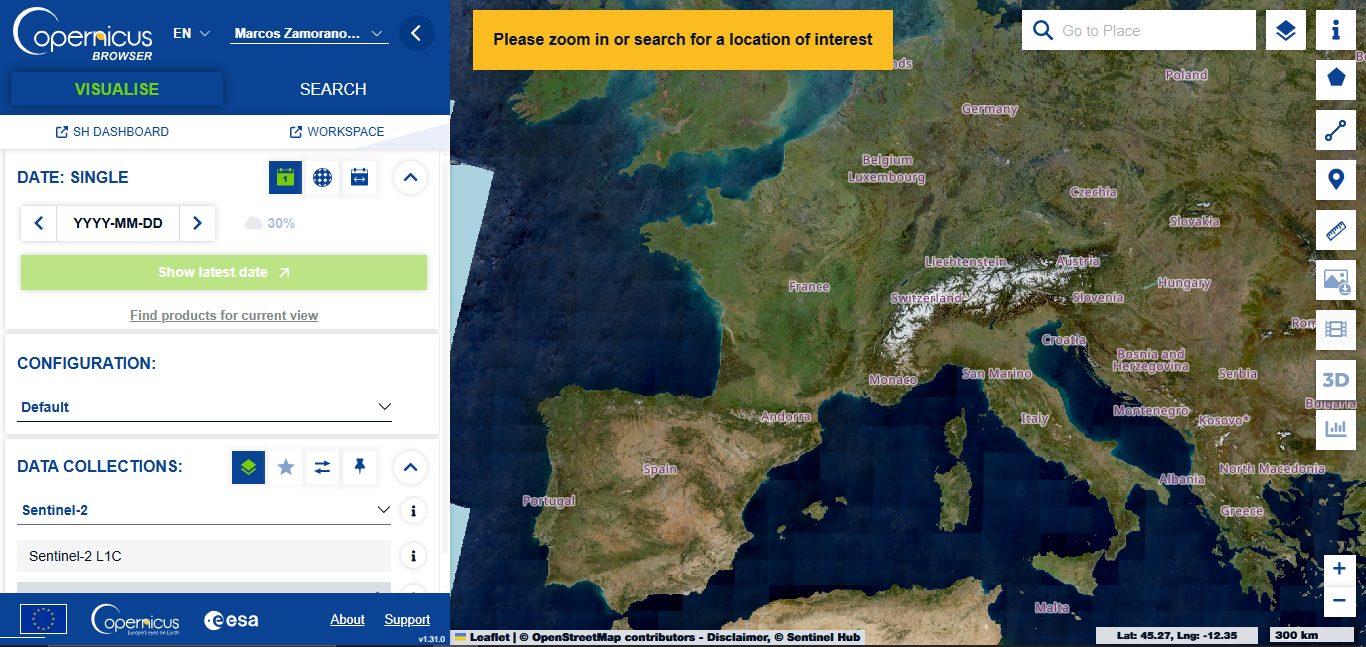
\includegraphics[width=0.7\linewidth]{Copernicus_Browser}
	\caption[Vista de la interfaz web de Copernicus Browser, mostrando un mosaico satelital en color real sobre Europa.]{}
	\label{fig:copernicus-browser}
\end{figure}


\item\textbf{Otras herramientas}

Además de las anteriores, cabe mencionar brevemente otras plataformas útiles según la finalidad: ESA SNAP, que consiste en un software de escritorio para procesado avanzado de imágenes de radar y ópticas, muy usado en investigación, Google Earth Pro, que permite la visualización 3D de imágenes históricas, aunque con limitaciones de resolución temporal en áreas naturales, NASA Worldview, un visor web de imágenes globales diarias, útil para ver rápidamente incendios, inundaciones u otros eventos, o visores regionales como el Centro de Descargas del CNIG en España. 

No obstante, para este proyecto centrado en sendas ecológicas, las herramientas ya descritas, QGIS, EarthExplorer, Sentinel Hub EO Browser y Copernicus Browser, cubren un espectro completo: desde el análisis GIS exhaustivo offline, pasando por la búsqueda masiva de datos brutos, hasta la visualización interactiva online. Integrar estas herramientas en el flujo de trabajo permitirá identificar, segmentar y validar las estructuras lineales de interés con mayor eficacia y rigor.
\end{itemize}

\capitulo{7}{Conclusiones y Líneas de trabajo futuras}

En este capítulo se recogen las conclusiones obtenidas tras la finalización del proyecto, valorando el grado de cumplimiento de los objetivos planteados, las principales decisiones tomadas durante el desarrollo y el aprendizaje técnico adquirido a lo largo del proceso. Asimismo, se incluyen posibles líneas de trabajo futuras, orientadas a ampliar las funcionalidades del sistema y mejorar su aplicabilidad en escenarios reales de análisis geoespacial.

\section{Conclusiones}

A continuación se sintetizan las principales conclusiones extraídas tras la finalización del proyecto:

\begin{itemize}
	\item Se han cumplido los objetivos establecidos inicialmente, trasladando la segmentación semántica de trazas de herbivoría a una aplicación web funcional. La solución permite cargar imágenes, ejecutar la detección, visualizar los resultados y gestionar flujos asociados a usuarios, colecciones geoespaciales y modelos.
	
	\item Se ha desarrollado una aplicación web monolítica modular con Flask, separando responsabilidades entre interfaz, lógica de aplicación, persistencia, procesamiento de imágenes e inferencia. Además del análisis de imágenes individuales, se ha incorporado soporte para visor cartográfico, generación de teselas, colecciones persistentes y procesamiento en segundo plano.
	
	\item Se ha diseñado un sistema extensible para la gestión de modelos, evitando que la aplicación dependa de uno único. Los administradores pueden incorporar modelos, validarlos antes de su uso y seleccionar cuál debe actuar como modelo activo, facilitando así la evolución futura del sistema.
	
	\item Ha sido necesario estudiar en profundidad tanto el código de ejecución del artículo base~\cite{diezpastora2025trails}, como el algoritmo proporcionado, analizando el flujo de preparación de imágenes, carga de modelos, ejecución de predicciones y generación de máscaras antes de adaptarlo a una aplicación con interacción real de usuario.
	
	\item Se han aplicado conocimientos adquiridos en distintas asignaturas del Grado en Ingeniería Informática, especialmente en \textit{Bases de Datos}, \textit{Análisis y Diseño de Sistemas}, \textit{Interacción Hombre-Máquina}, \textit{Gestión de Proyectos}, \textit{Estructuras de Datos}, \textit{Algoritmia}, \textit{Sistemas Inteligentes}, \textit{Minería de Datos} y \textit{Sistemas Distribuidos}.
	
	\item El proyecto también ha requerido adquirir nuevos conocimientos, principalmente en desarrollo web, peticiones y respuestas HTTP, gestión de sesiones, autenticación, autorización, formularios, renderizado con plantillas, comunicación mediante JSON, JavaScript, HTML, CSS y herramientas modernas de desarrollo.
	
	\item Uno de los retos principales ha sido transformar un entorno experimental, basado en un \textit{notebook} de inferencia, en una aplicación funcional capaz de gestionar errores, estados intermedios, usuarios, ficheros, modelos, permisos, procesos asíncronos y persistencia de resultados.
	
	\item Finalmente, se ha completado la documentación asociada al proyecto, incluyendo la memoria y los anexos. Esta tarea ha permitido justificar decisiones, ordenar conceptos, explicar alternativas y dejar constancia suficiente para facilitar la evaluación, mantenimiento y posible continuación del sistema.
\end{itemize}

\section{Líneas de trabajo futuras}

A partir del trabajo realizado, las líneas de mejora identificadas son las siguientes:

\begin{itemize}
	\item Una línea de mejora prioritaria sería estudiar la obtención de una licencia o autorización específica que permitiese integrar Google Earth Engine o fuentes de imaginería equivalentes bajo condiciones compatibles con el análisis automático. Esto permitiría trabajar con imágenes más próximas a aquellas utilizadas durante el entrenamiento del modelo original y, por tanto, mejorar la coherencia entre el dominio de entrenamiento y el dominio real de explotación.
	
	\item En la gestión de modelos, resultaría interesante incorporar un sistema de comparación visual entre predicciones generadas por las distintas opciones cargadas. Además de mostrar ambas segmentaciones sobre una misma imagen, podría añadirse una máscara de diferencias que resaltase los píxeles que cambian de un modelo a otro, facilitando así una decisión más informada sobre qué modelo debe configurarse como activo.
	
	\item En el visor cartográfico, una mejora útil consistiría en implementar un buscador por zona o localización. De esta forma, el usuario podría introducir un municipio, una coordenada o una referencia geográfica y desplazarse automáticamente a esa región del mapa, agilizando la selección de áreas de interés y mejorando la usabilidad del flujo geoespacial.
	
	\item También se plantea como trabajo futuro la incorporación de un sistema de notificaciones por correo electrónico. Este mecanismo permitiría avisar al usuario cuando finalice el procesamiento de una colección, especialmente en casos donde la segmentación de todas las teselas requiera varios minutos. Con ello se mejoraría la retroalimentación del sistema y se evitaría que el usuario tuviera que permanecer consultando manualmente el estado del proceso.
	
	\item Otra posible ampliación sería enriquecer el sistema de descarga de resultados, permitiendo exportar no solo las imágenes y los ficheros JSON de trazas, sino también informes automáticos en PDF o CSV con estadísticas agregadas de la colección, como número de teselas procesadas, longitud aproximada de trazas, área segmentada, errores detectados y modelo utilizado.
	
	\item Desde el punto de vista algorítmico, sería conveniente incorporar un módulo de evaluación asistida que permitiese comparar las trazas generadas con anotaciones manuales de referencia. Esto permitiría calcular métricas como \textit{IoU}, \textit{Dice}, \textit{accuracy}, \textit{recall} o $F_1$ sobre imágenes concretas, facilitando la validación de nuevos modelos y el análisis cuantitativo de su rendimiento en escenarios reales.
	
	\item Finalmente, aunque el sistema ya soporta procesamiento concurrente controlado mediante varios \textit{workers}, reclamación atómica de teselas y uso de SQLite como cola persistente, en escenarios de mayor carga podría evolucionarse hacia una cola de tareas especializada, como Redis o RabbitMQ. Esta migración permitiría incorporar mecanismos más avanzados de priorización, métricas de ejecución, paneles de monitorización, cancelaciones más finas y un escalado horizontal más robusto para contextos multiusuario o colecciones de gran tamaño.
\end{itemize}



\bibliographystyle{plain}
\bibliography{bibliografia}

\end{document}
